\documentclass[12pt]{article}

%Input preamble, math commands, environments, etc. from a saingle file. 
%Packages
\usepackage[top=1in, bottom=1in, left=.7in, right=.7in]{geometry}
\parindent 22pt
\usepackage{amsmath}
\usepackage{amsfonts}
\usepackage{amssymb}
\usepackage{bm}
\usepackage{etoolbox}
\usepackage{graphicx}
\usepackage{subfigure}
\usepackage{tabularx,ragged2e,booktabs}
\usepackage{caption}
\usepackage{hyphenat}
\usepackage{fixltx2e}
\usepackage[para]{threeparttable}
\usepackage[capposition=top]{floatrow}
\usepackage{pdfpages}
\usepackage{natbib}
\usepackage[colorlinks=true,linkcolor=blue,citecolor=blue]{hyperref}
\usepackage{setspace}
\doublespacing
\usepackage{rotating}

%Hyphens

%Environments
\newtheorem{theorem}{Theorem}[section]
\newtheorem{claim}[theorem]{Claim}
\newtheorem{assumption}[theorem]{Assumption}
\newtheorem{definition}[theorem]{Definition}
\newtheorem{hypothesis}[theorem]{Hypothesis}
\newtheorem{property}[theorem]{Property}
\newtheorem{example}[theorem]{Example}
\newtheorem{condition}[theorem]{Condition}
\newenvironment{proof}{\paragraph{Proof:}}{\hfill$\square$}

%Commands
\newcommand\independent{\protect\mathpalette{\protect\independenT}{\perp}}
\def\independenT#1#2{\mathrel{\rlap{$#1#2$}\mkern2mu{#1#2}}}
\newcommand{\overbar}[1]{\mkern 1.5mu\overline{\mkern-1.5mu#1\mkern-1.5mu}\mkern 1.5mu}
\newcommand{\equald}{\ensuremath{\overset{d}{=}}}













\begin{document}

\title{The Accumulation of Human Capital over the Life Cycle: Lessons from the Yoram Ben-Porath Model}
\author{Prepared by: Jorge L. Garc\'{i}a and Yike Wang \\ The University of Chicago}
\date{This Draft: \today}
\maketitle

\begin{flushright}
\textbf{Perhaps the most important conclusion to be drawn from research into the influence of income distribution on consumption is that the effects of inequality depend upon its causes. Mincer (1958).}
\end{flushright}


\begin{abstract}
\noindent For several years, economists have worried about theories of income and its prediction of observable outcomes or constructs of social interest. Particular interest they have paid to theories relating the distribution of income and the distribution of abilities (\citet{staehle1943ability} offers the first formal treatment on this topic in Economics). The most relevant ingredient of this analysis is human capital and its evolution. \citet{mincer1958investment} and \citet{becker1962investment} are the two main predecessors of the analysis of human capital investment. The former firstly asked why the distributions of abilities and income differed and argued for market compensation for different worker traits as principal causes. The latter established the first self-contained theoretical analysis of human capital investment. \citet{ben1967production} generalized \citet{becker1962investment} to a dynamic context that allows for a very rich analysis of the production of human capital. Specifically, it enables to analyze variations in (i) specialization periods; (ii) production functions of human capital; (iii) time horizons; (iv) rates of return. Based on the model in \citet{ben1967production}, we provide a framework to analyze the evolution of earnings and human capital under a wide variety of scenarios. We hope to guide researchers on the consequences of their human capital production and accumulation modeling choices.
\end{abstract}

\section{Basic Ben-Porath Model} \label{section:baseline}

The baseline Ben-Porath model studies how a single representative agent makes optimal life-cycle decisions on human capital investment to maximize her total lifetime disposable earnings. At each point in time, the agent's current stock of human capital, $H(t)$, and the rental rate of human capital, $R$, determine the amount of her potential earnings: $Y(t)=RH(t)$. The agent chooses two type of inputs in order to produce human capital: (i) a fraction of her current stock of human capital, $I(t)H(t)$, with $I(t) \in [0,1]$; (ii) market goods, $D(t)$. Therefore, the cost of human capital investments includes both foregone earnings, $RI(t)H(t)$, and cost of the purchased market goods, $P_DD(t)$, where $P_D$ is the price of the market goods.\\
\indent Then, the agent's disposable earnings in period $t$, $E(t)$, are equivalent to her potential earnings in period $t$, $Y(t)$, less the total costs:

\begin{equation}
E(t) = R H(t) -  R I(t) H(t) - P_{D} D(t) \label{eq:earnings}
\end{equation}

\indent The observed earnings the agent makes from her work in the labor market is $R(1-I(t))H(t)$, which are higher than her disposable earnings and lower than her potential earnings. Subtracting this by the cost of purchased market goods, $P_DD(t)$, gives her disposable earnings, $E(t)$.\\
\indent The agent produces human capital through a production function that takes two inputs.

\begin{assumption} (Strict Concavity of the Production Function) \label{assumption:scpf}  $\forall \ t \in [0,T] \ F(\cdot, \cdot)$ is strictly concave in both of its arguments.
\end{assumption}

\indent The change in human capital stock at time $t$, which is summarized by the law of motion for $H(t)$, is defined as: 

\begin{definition} (Law of Motion for Human Capital Stock in the Basic Ben-Porath Specification)
\begin{equation}
\dot{H(t)} = F \left( I(t) H(t), D(t) \right) - \sigma H(t). \label{eq:lawh}
\end{equation}
\end{definition}

\indent The law of motion for human capital stock embeds a neutrality assumption. Namely, the current stock of human capital at time $t$, $H(t)$, and the investment time at time $t$, $I(t)$, appear as a single argument in a multiplicative form in the flow production of human capital stock. This assumption simplifies our calculations by neutralizing the effect of $H(t)$ on the optimal decision of time investment. In particular, a higher level of $H(t)$ increases the marginal return of $I(t)$ in producing human capital and the marginal cost of $I(t)$ in foregone earnings, both in a multiplicative pattern. As a result, $H(t)$ cancels out in the first order condition for $I(t)$ as we show later.\\
\indent The agent's life-cycle problem is to choose $I(t)$ and $D(t)$ over time to maximize her total disposable earnings subject to the law of motion for human capital. Given an initial condition of human capital, $H(0)=H_0$, the agent's problem is as follows.

\begin{problem} \label{problem:bbp} (Life-cycle Individual's Problem in the Basic Ben-Porath Model)
\begin{equation}
\max_{{I_{t}, D_{t}}} \int \limits _{0} ^{T} \exp^{-rt} RH(t)(1 - I(t)) dt \nonumber \\
\end{equation}
\noindent s.t.
\begin{eqnarray}
H(0) &=& H_{0} \nonumber \\
\dot{H(t)} &=& F \left( I(t) H(t), D(t) \right) - \sigma H(t) \nonumber
\end{eqnarray}
\end{problem}

\indent Therefore, the current value Hamiltonian associated to the agent's maximization problem is
\begin{equation}
\mathcal{H} (\cdot) = \exp^{-rt} \left[ R H(t) -  R I(t) H(t) - P_{D} D(t) \right] + \mu(t) \dot{H(t)} 
\end{equation}

\noindent where $\mu(t)$ defines the shadow price of the human capital stock. Thus, the following conditions must be satisfied for the interior solution.

\begin{condition} (Optimality Conditions for the Life-cycle Individual's Problem in the Basic Ben-Porath Model) 
\begin{eqnarray}
\frac{\partial \mathcal{H} (\cdot)}{\partial I(t)} = 0 &\Leftrightarrow& \exp^{-rt}R = \mu(t) F_{1} \left( I(t) H(t), D(t) \right) \label{eq:focinvestment} \\
\frac{\partial \mathcal{H} (\cdot)}{\partial D(t)} = 0 &\Leftrightarrow& \exp^{-rt}P_D = \mu(t) F_{2} \left( I(t) H(t), D(t) \right) \label{eq:focgoods} \\
\frac{\partial \mathcal{H} (\cdot)}{\partial H(t)} = - \dot{\mu(t)} &\Leftrightarrow& \exp^{-rt} R \left( 1 - I (t) \right) + \mu(t) \left(  F_{1} \left( I(t) H(t), D(t) \right)I(t) - \sigma \right) = - \dot{\mu(t)} \label{eq:focstock} \\ 
\frac{\partial \mathcal{H} (\cdot)}{\partial \mu(t)} = \dot{H(t)} &\Leftrightarrow& \dot{H(t)} = F \left( I(t) H(t), D(t) \right) - \sigma H(t) \label{eq:focmotion} \\
\text{Transversality} &:& \lim_{t \rightarrow T} \mu(t) H(t) = 0 \label{eq:foctransversality}
\end{eqnarray}
where $F_j$ is the first order derivative of the production function $F$ with respect to argument $j$.
\end{condition}

\indent To simplify notation, combine the two terms with intertemporal meaning in the life-cycle decision problem into one term through $g(t)\equiv \exp^{rt}\mu(t)$. Then, combine \eqref{eq:focinvestment} and \eqref{eq:focstock} to get 
\begin{equation}
\dot{\mu(t)} = - \exp^{-rt} R + \mu(t) \sigma \label{eq:focinvstockcombine}
\end{equation}

\noindent and note that $\dot{g(t)} = \dot{\mu(t)} \exp^{rt} + r \mu(t) e ^{rt}$. Use \eqref{eq:focinvstockcombine} to obtain 
\begin{equation}
\dot{g(t)} = (\sigma + r ) g(t) - R. \label{eq:grossdep}
\end{equation}

\indent Equation~\eqref{eq:foctransversality} implies that $\mu(T) = 0 $, and therefore $g(T) = 0$ provided that $H(T) = 0$ has no economic sense.% that last clause doesn't make sense
 It is possible, thus, to solve \eqref{eq:grossdep} and obtain
\begin{equation}
g(t) = \frac{R}{\sigma + r} \left[ 1 - \exp^{(\sigma + r)(t - T)} \right],
\end{equation}

\noindent which leads to $\dot{g(t)} < 0$. To wrap up the discussion, note that the optimality conditions for the interior solution are:
\begin{eqnarray}
g(t) F_{1}(I(t)H(t),D(t)) &=& R \nonumber \\
g(t) F_{2}(I(t)H(t),D(t)) &=& P_{D} \label{eq:newfocs}. 
\end{eqnarray}

\indent The system in \eqref{eq:newfocs} consists of two equations and two unknowns that solve for the Marshallian demand for $I(t)H(t)$ and $D(t)$. Note that if the optimal solutions are interior and the cross-partial derivative of the production function with respect to its two arguments is assumed to be zero, i.e. $\frac{\partial^2F}{\partial IH \partial D} = 0$, strict concavity of the production function together with $\dot{g(t)} < 0$ imply that both Marshallian demands are decreasing overtime. This is intuitive, because the agent faces a finite horizon problem and the amount of time left to capture the returns of human capital investment decreases over time. 

\subsection{Earnings Dynamics}
\indent One important question this basic model enables us to ask is how earnings evolve over the life-cycle. Consider both the slope and curvature of the earnings dynamics in the case with no $D(t)$, i.e. $F_{D(t)}=0$ so that the production function takes the single argument $I(t)H(t)$. Without loss of generality, also assume that $R\equiv1$.

\subsubsection{The Slope of Earnings Dynamics}

\begin{claim} (Earnings over Time with no Depreciation) \label{claim:earnnodep}
Let $\sigma = 0$. Then, when the optimal solution for $I(t)$ is interior, $\dot{E(t)} > 0$.
\end{claim}

\begin{proof}
Differentiate \eqref{eq:earnings} and use \eqref{eq:lawh} to write
\begin{eqnarray}
\dot{E(t)} &=& \dot{H(t)} - \dot{I(t)H(t)}  \nonumber \\
           &=& F \left( I(t) H(t) \right) - \dot{I(t)H(t)}  \nonumber \\     
           &>& 0 
\end{eqnarray}

\noindent where the inequality follows because the Marshallian demands for $I(t)H(t)$ is decreasing over time.
\end{proof}

\begin{claim} (Earnings over Time with Depreciation) \label{claim:earndep}
Let $\sigma > 0$. Then, $\dot{E(t)} \lessgtr 0$. 
\end{claim}

\begin{proof}
Follow the same steps as in the proof of Claim~\ref{claim:earnnodep} and note that the term $\sigma H(t)$ appears in the expression for $\dot{E(t)}$. This term could be $\lessgtr F \left( I(t) H(t) \right) - \dot{I(t)H(t)} $.
\end{proof}

\indent Claim \ref{claim:earnnodep} follows because with a positive amount of investment (interior solution) and no depreciation, human capital stock accumulates over time. Moreover, investment in human capital declines over time, and thus disposable earnings increase over time. Claim \ref{claim:earndep} follows because the accumulated stock of human capital may be driven down by a relatively high rate of depreciation.

\subsubsection{The Curvature of Earnings Dynamics} \label{section:egdyn}
\indent We now analyze the curvature of the earnings function for the case in which there is no depreciation.\footnote{A similar analysis follows when $\sigma>0$ for the cases in which either $\dot{E(t)}> 0$ or $\dot{E(t)}< 0$}. 

\begin{claim} (Concavity of the Earnings Function with no Depreciation)
\label{claim:concearnnodep}
Assume that $\eta \equiv \left( 1 - \frac{F'F'''}{{F''}^2} \right) < 0$. Then, the earnings function is strictly concave. 
\end{claim}

\begin{proof}
First note that $\dot{E(t)} > 0$ by Claim~\ref{claim:earnnodep}. Since $F_{D(t)} = 0 $ we can write the first order condition for investment as
\begin{equation}
g(t) F'(I(t) H(t)) = 1
\end{equation}
and differentiate it with respect to $t$ to get
\begin{eqnarray}
\dot{g(t)} F'(I(t) H(t)) + g(t) F''(I(t) H(t)) \dot{I(t) H(t)} &=& 0 \nonumber \\
&\Leftrightarrow& \nonumber \\
\dot{I(t) H(t)} &=& - \left( \frac{\dot{g(t)}}{g(t)} \right) \left[ \frac{F'}{F''}\right] \label{eq:itdot}.
\end{eqnarray}
\noindent Moreover, drop the argument $t$ to shorten notation, and note that
\begin{eqnarray}
\ddot{IH} = - \left[ \frac{\ddot{g}}{g} - \left( \frac{\dot{g}}{g} \right)^2 \right] \frac{F'}{F''} + \left( \frac{\dot{g}}{g} \right)^2 \left[ 1 - \frac{F'F'''}{{F''}^2} \right] \left[ \frac{F'}{F''} \right]  
\end{eqnarray}  
where we substitute in $\eqref{eq:itdot}$. Further, note that
\begin{eqnarray}
\dot{E} &=& F(IH) - \dot{IH} - \sigma H \nonumber \\
\ddot{E} &=& F'(IH) \dot{IH} - \ddot{IH} - \sigma \dot{H} \nonumber \\
&=& \frac{1}{g} \dot{IH} - \ddot{IH} - \sigma \dot{H}.
\end{eqnarray}

\noindent and from \eqref{eq:grossdep} obtain $\frac{\ddot{g}}{g} = r \frac{\dot{g}}{g}$. Thus,
\begin{eqnarray}
\ddot{E} &=& - \frac{\dot{g}}{g} \frac{F'}{F''} \left[ \frac{1}{g} + \frac{\dot{g}}{g} \left( 1 - \frac{F'F'''}{{F''}^2} \right) \right] + \left[ r \frac{\dot{g}}{g} - \left( \frac{\dot{g}}{g} \right)^2 \right] \frac{F'}{F''} \nonumber \\
&=& - \frac{\dot{g}}{g} \frac{F'}{F''} \left[ \frac{1}{g} + \frac{\dot{g}}{g} \left( 1 - \frac{F'F'''}{{F''}^2} \right) - \frac{gr - \dot{g}}{g} \right] \nonumber \\
&=& - \frac{\dot{g}}{g} \frac{F'}{F''} \left[ \frac{1}{g} + \frac{\dot{g}}{g} \left( 1 - \frac{F'F'''}{{F''}^2} \right) - \frac{1}{g} \right] \nonumber \\
&=& - \left( \frac{\dot{g}}{g} \right)^2 \frac{F'}{F''} \left( 1 - \frac{F'F'''}{{F''}^2} \right)
\end{eqnarray}

\noindent where the third equality uses \eqref{eq:grossdep}, i.e. $gr - \dot{g} = 1$. F is strictly concave and therefore $-\left( \frac{\dot{g}}{g} \right)^2 \frac{F'}{F''} > 0$. Since $\left( 1 - \frac{F'F'''}{{F''}^2} \right) < 0$ the claim follows.
\end{proof}

\indent  Therefore, ${E(t)}$ is concave if and only if $\eta < 0$, which implies a necessary condition for concavity: $F^{'''}>0$.

\begin{example} (Human Capital Production Functions and Earnings Concavity)
\begin{itemize}
\item Power Production Function 1 : consider the case of $F(x) = \frac{Ax^{\alpha}}{\alpha}$ for $ - \infty < \alpha < 1, A > 0$. Then, $\eta = \frac{1}{\alpha - 1} < 0$. Under this specification the earnings function is strictly concave with respect to time.
\item Power Production Function 2 : consider the case of $F(x) = a - b x ^ {- \alpha}$ for $ - 1 < \alpha < \infty, a,b,c > 0$. Then, $\eta = \frac{-1}{\alpha + 1} < 0$. Under this specification the earnings function is strictly concave with respect to time.
\item Power Production Function 3: consider the case of $F(x) = a - b \exp^{-cx}$ with $b,c > 0$. Then, $\eta = 0$. 
\item Quadratic Production Function: any quadratic production function has $F''' = 0$ and does not induce concavity of earnings with respect to time. 
\end{itemize}
\noindent Note, all of these examples consider no depreciation of human capital, $\sigma = 0$. 
\end{example} 

\subsection{The Specialization Period} \label{section:specialization}
Specialization happens when the agent devotes her entire human capital to produce human capital stock, i.e. when $I(t) = 1$ for $t \in [ \underline{t}, \bar{t}]$. In order to analyze some of the properties of specialization periods we assume away $D(t)$ so that $F_{D(t)} = 0$ and rule out depreciation.\\
\indent Recall that we can interpret $g(t)$ as the return to investment in human capital and that we show above that $\dot{g} < 0$. Then, there is at most one period of specialization at the beginning of the time horizon, if it happens. We denote this by $[0,t^*]$. \citet{ben1967production} calls this the schooling period and it happens under the conditions that follow.

\begin{condition} (Conditions for the Existence of a Period of Specialization in the Basic Ben-Porath Model with no Depreciation)
\begin{eqnarray}
F'(H(t))g(t) &>& R\ \ \ \forall \ t\in [0,t^*) \nonumber \\
F'(H(t^*))g(t^*) &=& R\nonumber \\
I(t) &=& 1\ \ \ \ \forall \ t\in [0,t^*] \nonumber \\
H(t^*) &=& \int \limits _{0} ^{t^*} F (H(\tau)) d\tau + H_{0} \label{eq:humantstar}
\end{eqnarray} 
\noindent where $H(t^*)$ is the human capital stock accumulated up to time $t^*$.\\
\end{condition}

\indent Given that $R$ is fixed, any decrease in the function $g(t)$ for a given $t$ lowers $t^*$ because it lowers the return to gross investment in human capital. For example, relatively high $r$ implies relatively low $t^*$ because the individual is relatively present oriented. % present oriented sounds weird, change it
 Also, from the system \eqref{eq:humantstar}, note that a high value of $H_0$ implies a lower value for $t^*$ because it takes less time to obtain $H(t^*)$. If $\sigma > 0 $, similar conditions characterize the specialization period. However, there may be more than one specialization period because, under some scenarios, a high value of $\sigma$ may knock off capital such that various investment episodes are optimal. We defer that case for Section \ref{section:cycles}.
\begin{case} (No Depreciation and the Cobb-Douglas Production Function for Human Capital: Initial Level of Human Capital) \label{case:ndcdexample}
In this case $\dot{H} = A \left(IH \right)^\alpha$ where $0 < \alpha < 1, A>0$. As argued above, if it exists, specialization happens in the period $[0,t^*]$. Thus
\begin{eqnarray}
	\alpha A \left( H(0) \right) ^{\alpha - 1 }g(0) &>& R \nonumber \\
	&\Leftrightarrow& \nonumber \\
	H(0) &<& \left[ \frac{R}{g(0)\alpha A} \right]^{\frac{1}{\alpha-1}} \label{eq:h0forspe}.
\end{eqnarray}
\indent As the conditions in \eqref{eq:humantstar} establish, the time spent in specialization is a decreasing function of $H(0)$. In this example, actually, the initial human capital needs to be below certain threshold in order for the individual to specialize during one period. 
\end{case}

\begin{case} (No Depreciation and the Cobb-Douglas Production Function for Human Capital with Infinite Horizon: Initial Level of Human Capital)
In the setting of Case~\ref{case:ndcdexample} and if the horizon of the problem is infinite: $H(0) < \left( \frac{\alpha A}{r} \right) ^{\frac{1}{1 - \alpha}}$ because $g(t) = \frac{R}{r}$.
\end{case}

\begin{case} (No Depreciation and the Cobb-Douglas Production Function for Human Capital: the Specialization Period)
In the period of specialization $I(t) = 1$. Then,
\begin{equation}
\dot{H} = A \left( H \right)^{\alpha} \label{eq:humandiff}.
\end{equation}
The general solution for \eqref{eq:humandiff} is
\begin{equation}
H(t) = \left[ (1 - \alpha)(At + K) \right]^{\frac{1}{1-\alpha}}
\end{equation}
for some constant $K$. Given an initial condition $H(0) = H_{0}$, $K = \frac{H_{0}^{1-\alpha}}{1-\alpha}$ and
\begin{equation}
H(t) = \left[ (1 - \alpha)At + H_{0}^{1-\alpha} \right]^{\frac{1}{1-\alpha}} \label{eq:hbeforetstar}.
\end{equation}
At the end of the specialization period, as established in \eqref{eq:humantstar}:
\begin{equation}
\alpha g(t^*) A \left( H(t^*) \right)^{\alpha - 1} = R.
\end{equation}
If $T \rightarrow \infty$, $g(t) = \frac{R}{r}$ and
\begin{equation}
t^* = - \frac{H_{0}^{1 - \alpha}}{A(1 - \alpha)} + \frac{\alpha}{1 - \alpha}\frac{1}{r}. \label{eq:tstar}
\end{equation}

\indent \eqref{eq:tstar} provides some intuitive results: (i) an individual with relatively high initial human capital specializes during a relatively shorter period: $\frac{\partial t^*}{\partial       H_{0}} < 0$; (ii) a relatively able individual specializes during relatively long period: $\frac{\partial t^*}{\partial A} > 0$; (iii) a relatively impatient individual specializes for a relatively shorter period: $\frac{\partial t^*}{\partial r} < 0$.
% you can't say relatively abler or relatively longer
% it's EITHER relatively able OR abler
% it's redundant to say both. Personally I'd go through a remove all the 'relatively's
\end{case}

\begin{case} (No Depreciation and the Cobb-Douglas Production for Human Capital: Post-school Earnings)
Let $\tau = t - t^*$ define the post-school work experience and write post-school earnings as follows:
\begin{equation}
E(\tau) = R \int \limits _{0} ^{\tau} \dot{H( l + t^*)}d l + R H(t^*) - RIH(\tau + t^*).
\end{equation}
Now, from \eqref{eq:humantstar} the following equality holds:
\begin{eqnarray}
\alpha g(t) A \left( IH(t) \right)^{\alpha - 1} &=& R \nonumber \\
&\Leftrightarrow& \nonumber \\
IH(t) &=& \left[ \frac{\alpha g(t) A}{R} \right]^{\frac{1}{1-\alpha}} \label{eq:itcobb}
\end{eqnarray}
Combining \eqref{eq:itcobb} and the law of motion for human capital:
\begin{equation}
\dot{H} = A \left[ \frac{\alpha g(t) A}{R} \right]^{\frac{\alpha}{1-\alpha}} \label{eq:hdot}.
\end{equation}
Then,
\begin{equation}
E(\tau) = R \int \limits _{0} ^{\tau} A \left[ \frac{\alpha g(l + t^*) A}{R} \right]^{\frac{\alpha}{1-\alpha}} dl + RH(t^*) - R \left[ \frac{\alpha g \left( \tau + t^* \right) A}{R} \right]^{\frac{1}{1-\alpha}} \label{equation:postearnings}
\end{equation}
and if $T \rightarrow \infty$
\begin{equation}
E(\tau) = RA \left[ \frac{\alpha A}{r} \right]^{\frac{\alpha}{1-\alpha}} \tau.
\end{equation}

\begin{center}
\begin{figure}[H]
\caption{Earnings and Experience, Cobb Douglas Technology and No Depreciation}
\centering
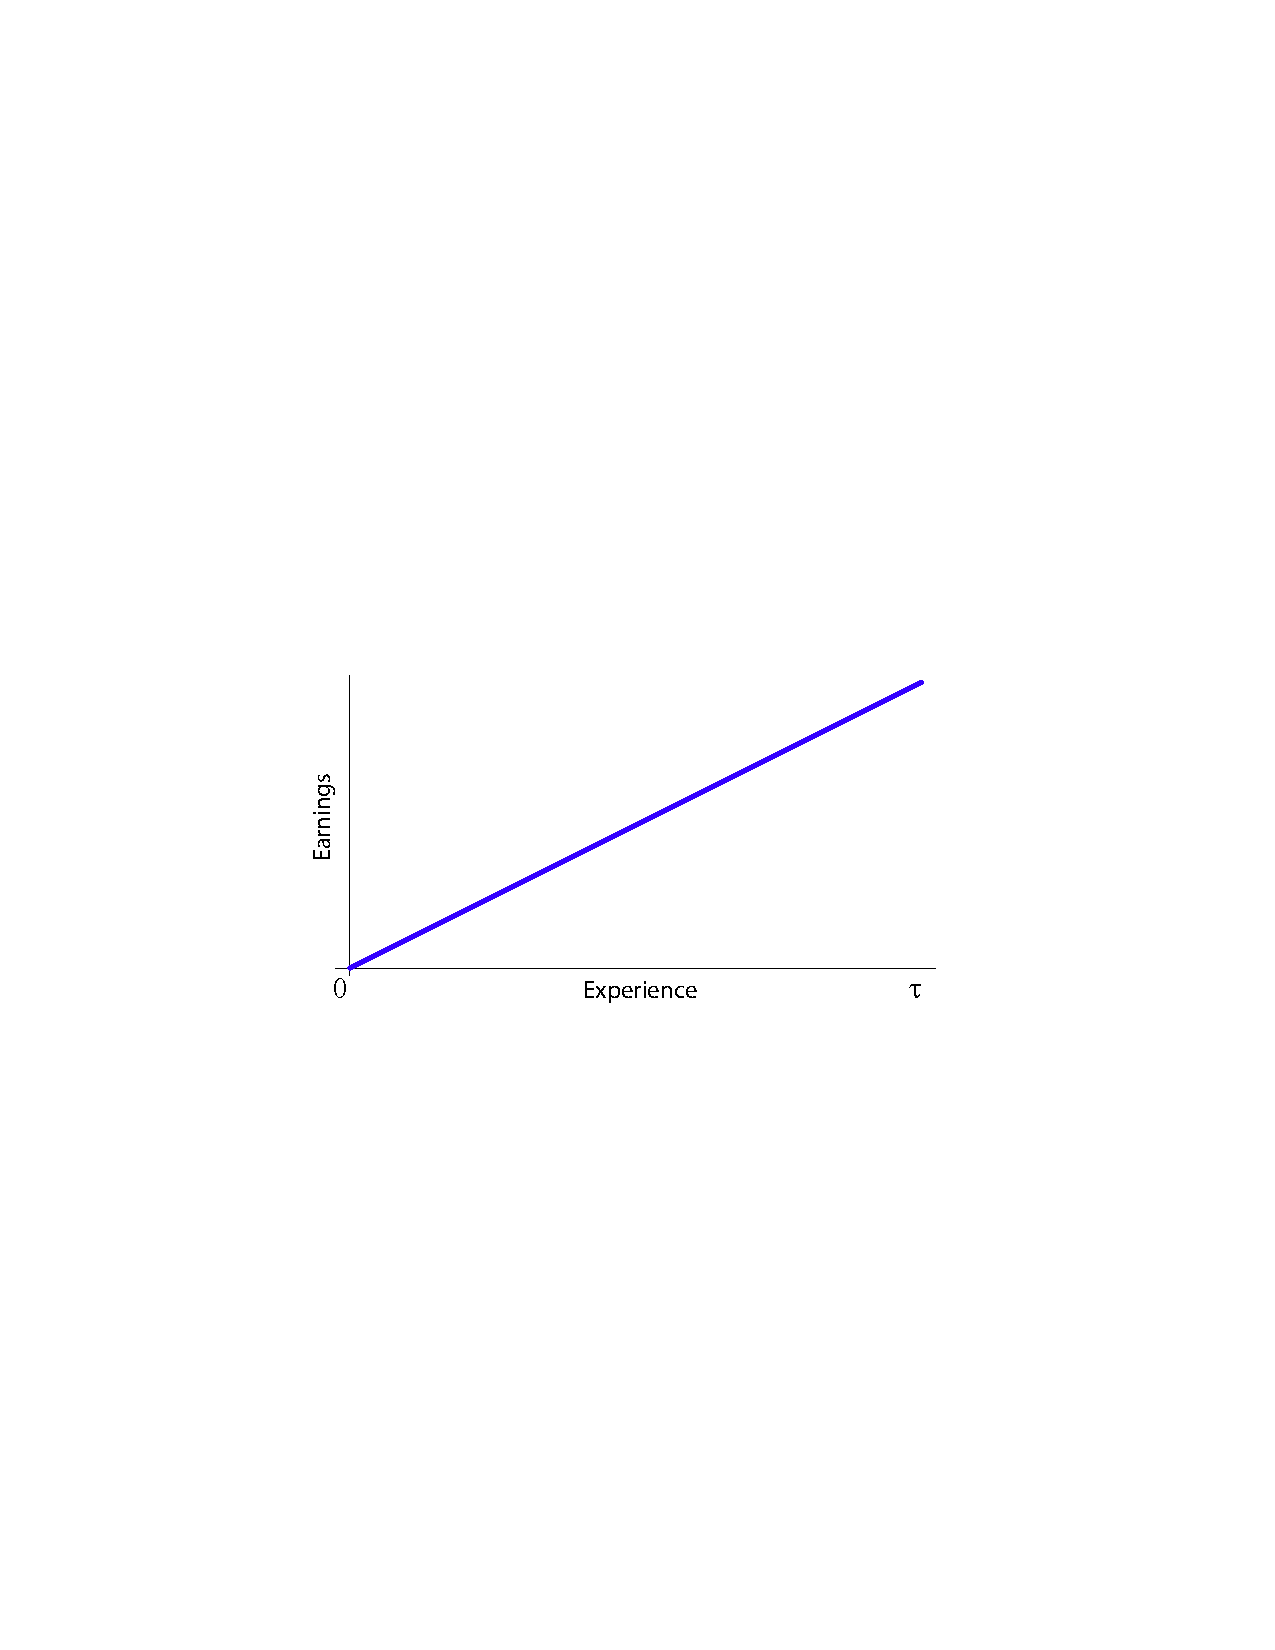
\includegraphics[width=3.5in, height=1.5in]{Figures/fig-earnings-experience.pdf}
\end{figure}
\end{center}

\indent When the time horizon is infinite, there is no concern with the reduction in time left for capturing returns to human capital investment and thus $g(t)$ is fixed over time. When the solution is interior, the optimal choice on $I(t)H(t)$ is constant overtime, which implies the increase in $H(t)$ overtime is also a constant. This is why $E(t)$ increases at a constant rate as well. However, with a finite time horizon, the Cobb-Douglas production function with no depreciation implies a strictly concave earning function $E(t)$.
\end{case}

\subsection{The Baseline Model Dynamics under the Cobb-Douglas Specification: a Summary}
This section summarizes the dynamics of the main variables in the baseline model when there is no depreciation, market goods are ruled out, and the production function for human capital investment is Cobb-Douglas. We assume that the horizon is infinite to simplify the algebra, but it is important to note that the qualitative properties of the results remain unchanged under a finite horizon. To wrap up the section, we show simulations that illustrate how the variables of interest behave under various parameterizations (in all of them we set $R = 1$). 

\subsubsection{Human Capital}
\begin{itemize}
\item At $t = 0$ an initial condition is given.
\item At $0 < t < t^*$ the system \eqref{eq:humantstar} provides the conditions that human capital satisfies and its expression is given by \eqref{eq:hbeforetstar}.
\item At $t = t^*$ \eqref{eq:hbeforetstar} is still a valid expression for human capital. To obtain the exact quantity it suffices to substitute the expression for $t^*$, \eqref{eq:tstar}, into \eqref{eq:hbeforetstar}.
\item At $ t > t^* $ \eqref{eq:humantstar} and the expression for $\dot{H}$, \eqref{eq:hdot}, provide the expression for human capital.
\end{itemize}

Then,

\begin{eqnarray}
H(t) =
\begin{cases}
H_{0} & t = 0 \\
\left[ (1 - \alpha)At + H_{0}^{1-\alpha} \right]^{\frac{1}{1-\alpha}} , & 0 < t < t^* \\
\left[ \frac{\alpha A}{r} \right]^{\frac{1}{1 - \alpha}}, & t = t^* \\
A \left[ \frac{\alpha A}{r} \right]^{\frac{ \alpha }{1 - \alpha}} \left( t - t^* \right) + \left[ \frac{\alpha A}{r} \right]^{\frac{1}{1 - \alpha}} , & t > t^*. \label{eq:humancapall}
\end{cases}
\end{eqnarray}

\subsubsection{Investment}
We focus on the case in which there is an specialization period, i.e. the case in which \eqref{eq:h0forspe} holds. The combination of \eqref{eq:itcobb} and \eqref{eq:humancapall} gives the following

\begin{eqnarray}
I(t) =
\begin{cases}
1, & t = 0 \\
1, & 0 < t < t^* \\
1, & t = t^* \\
\frac{\left[ \frac{\alpha A}{r} \right]^{\frac{1}{1 - \alpha}}}{A \left[ \frac{\alpha A}{r} \right]^{\frac{ \alpha }{1 - \alpha}} \left( t - t^* \right) + \left[ \frac{\alpha A}{r} \right]^{\frac{1}{1 - \alpha}}}, & t > t^*. \label{eq:investall}
\end{cases}
\end{eqnarray}

\subsubsection{Earnings}
For earnings we also focus on the case with a specialization period, i.e. the case in which \eqref{eq:h0forspe} holds. Thus, \eqref{eq:earnings}, \eqref{eq:humancapall}, \eqref{eq:investall} define earnings as follows

\begin{eqnarray}
E(t) =
\begin{cases}
0, & t = 0 \\
0, & 0 < t < t^* \\
0, & t = t^* \\
RA \left[ \frac{\alpha A}{r} \right]^{\frac{\alpha}{1 - \alpha}} \left( t - t^* \right) , & t > t^*. \label{eq:earnsall}
\end{cases}
\end{eqnarray}

\begin{figure}[H]
\centering
\captionsetup{justification=centering}
    			\caption{Dynamics with Variations in a Production Technology Parameter\\
    			$\alpha = .3$ (dotted); $\alpha = .4$ (dashed); $\alpha = .5$ (solid) \\
    			 for  $A = 3, r = .05, H_{0} = 1$ \\  }
        \subfigure[Human Capital Investment]{
            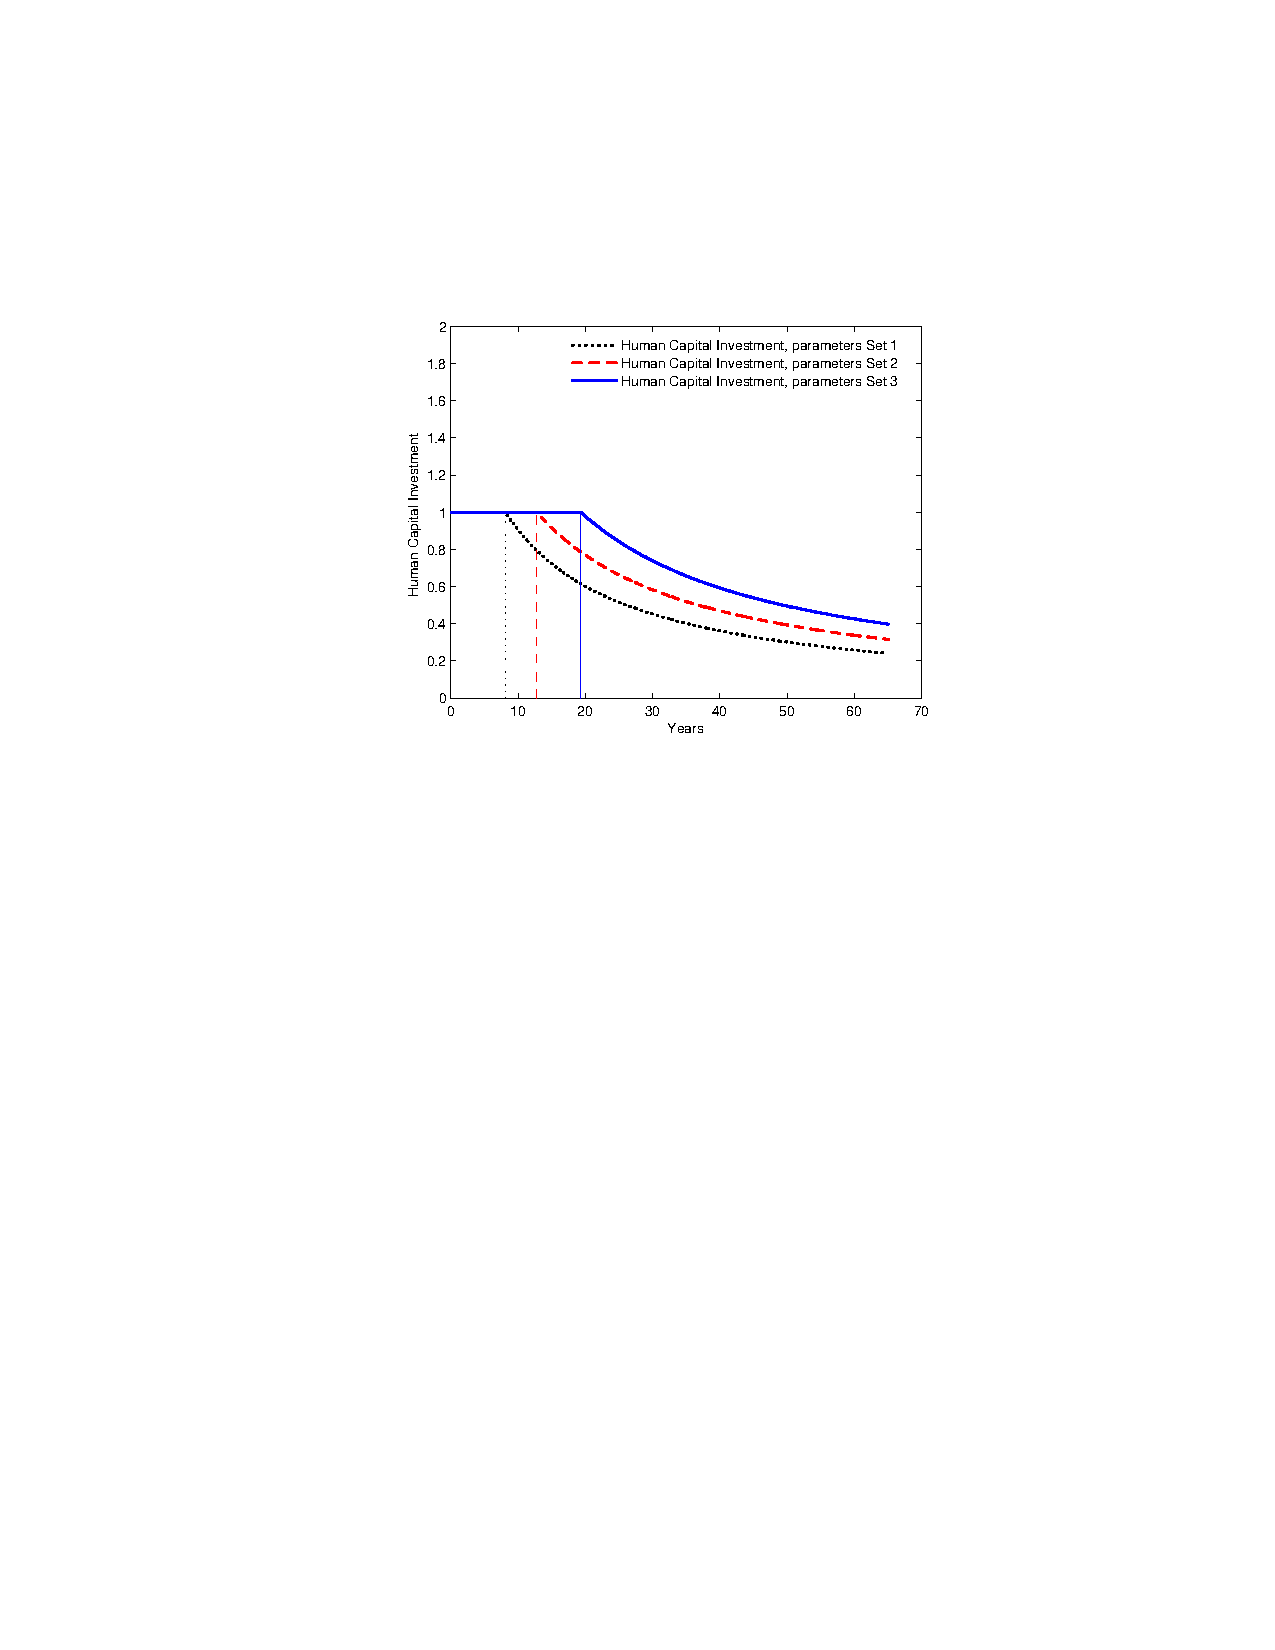
\includegraphics[width=2.2in, height=2.2in]{Figures/fig-hc-earn-series-02.pdf}
        }\\
        \subfigure[Human Capital Stock]{
            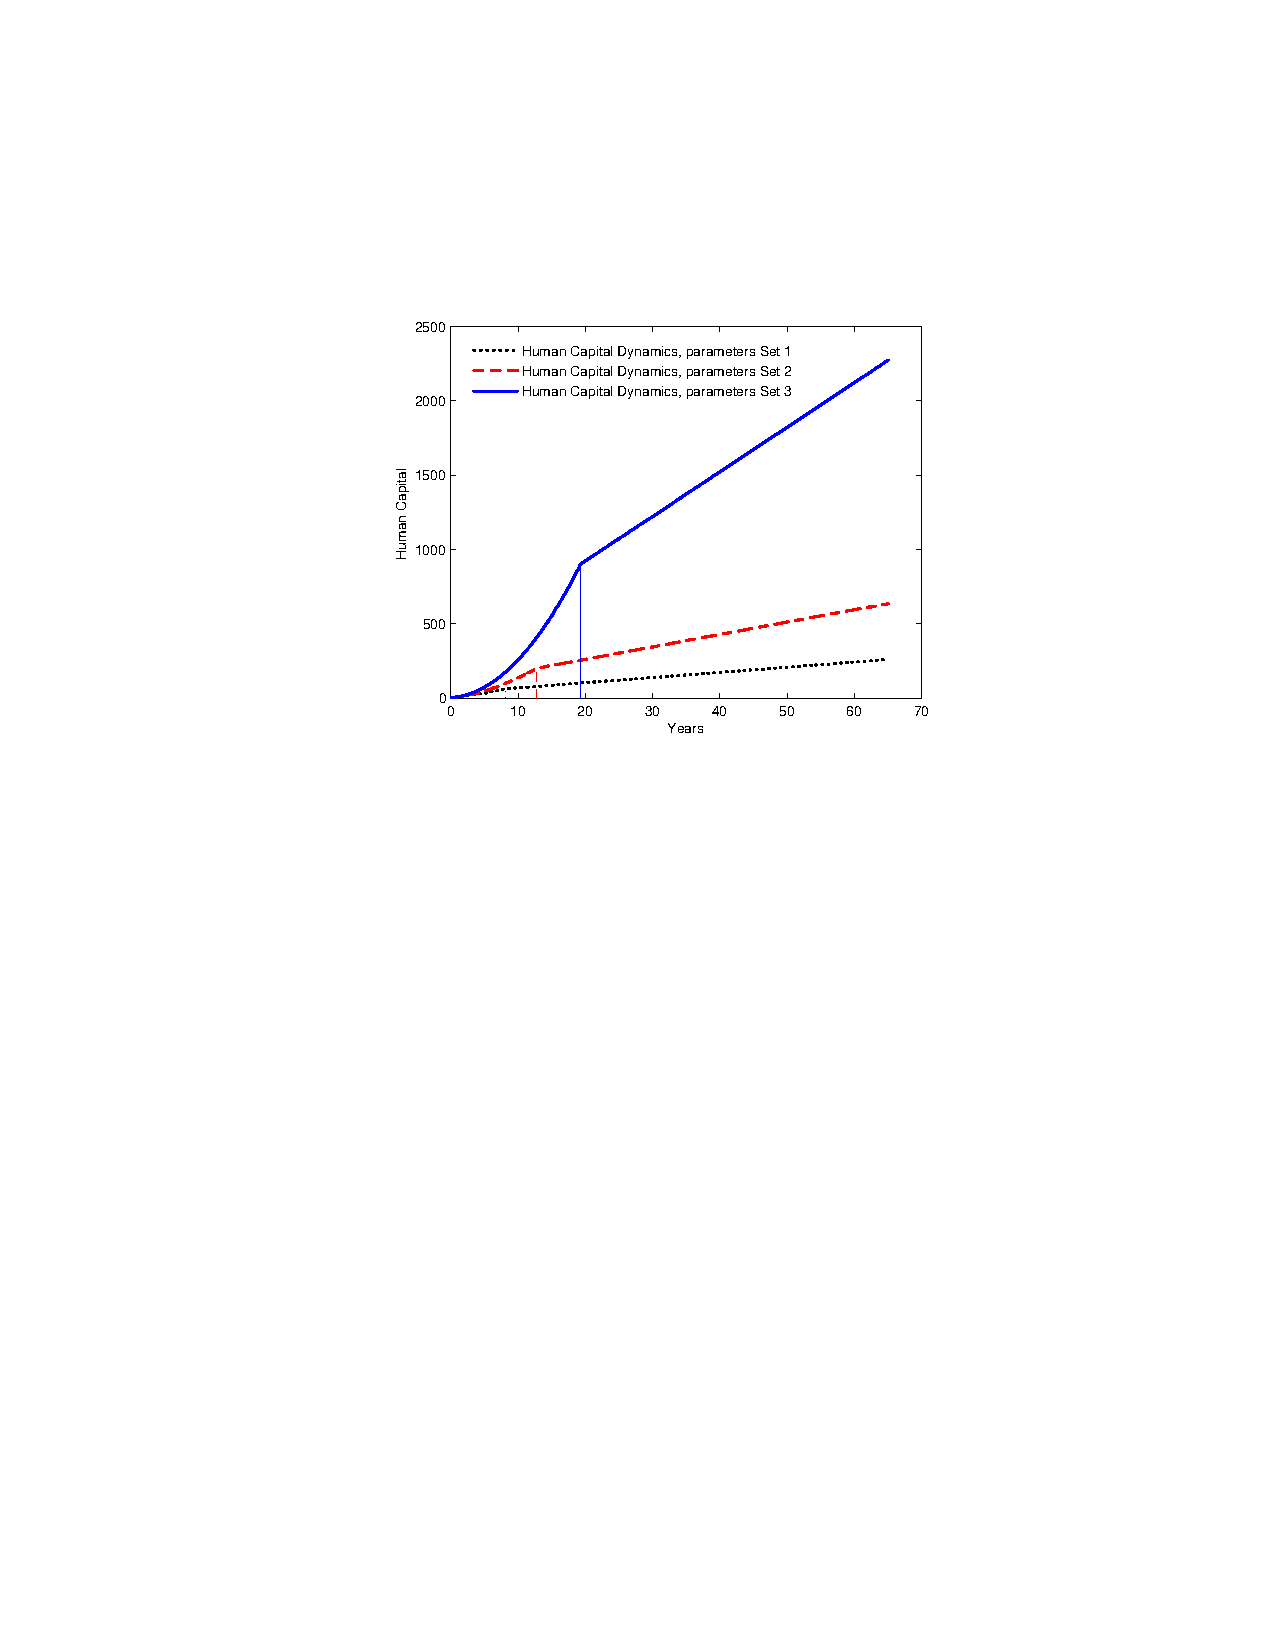
\includegraphics[width=2.2in, height=2.2in]{Figures/fig-hc-earn-series-01.pdf}
        }\\
        \subfigure[Earnings]{%
            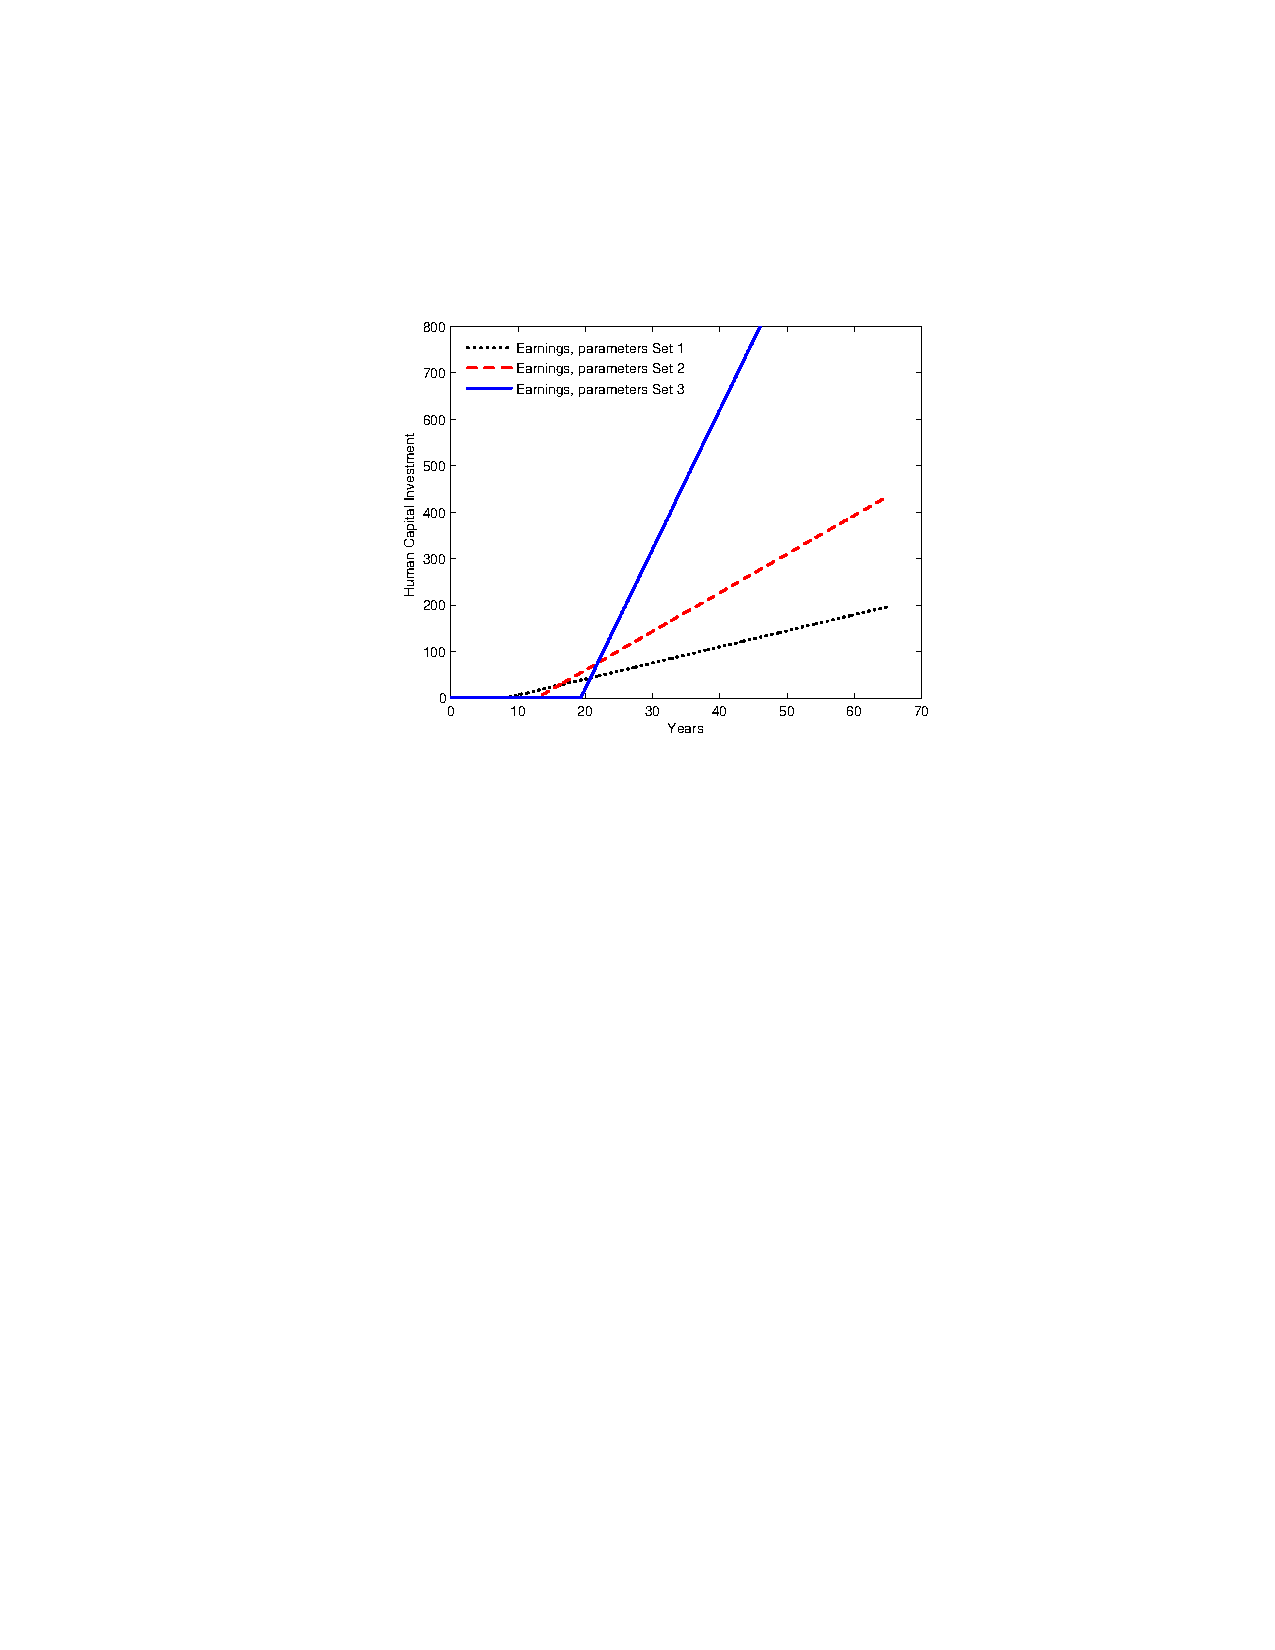
\includegraphics[width=2.2in, height=2.2in]{Figures/fig-hc-earn-series-03.pdf}
        }
\end{figure}

\begin{figure}[H]
\centering
\captionsetup{justification=centering}
    			\caption{Dynamics with Variations in the Discounting Factor \\
    			$r = .04$ (dotted); $r = .05$ (dashed); $r = .06$ (solid) \\
    			for $A = 3, \alpha = .5, H_{0} = 1$ \\  }
        \subfigure[Human Capital Investment]{
            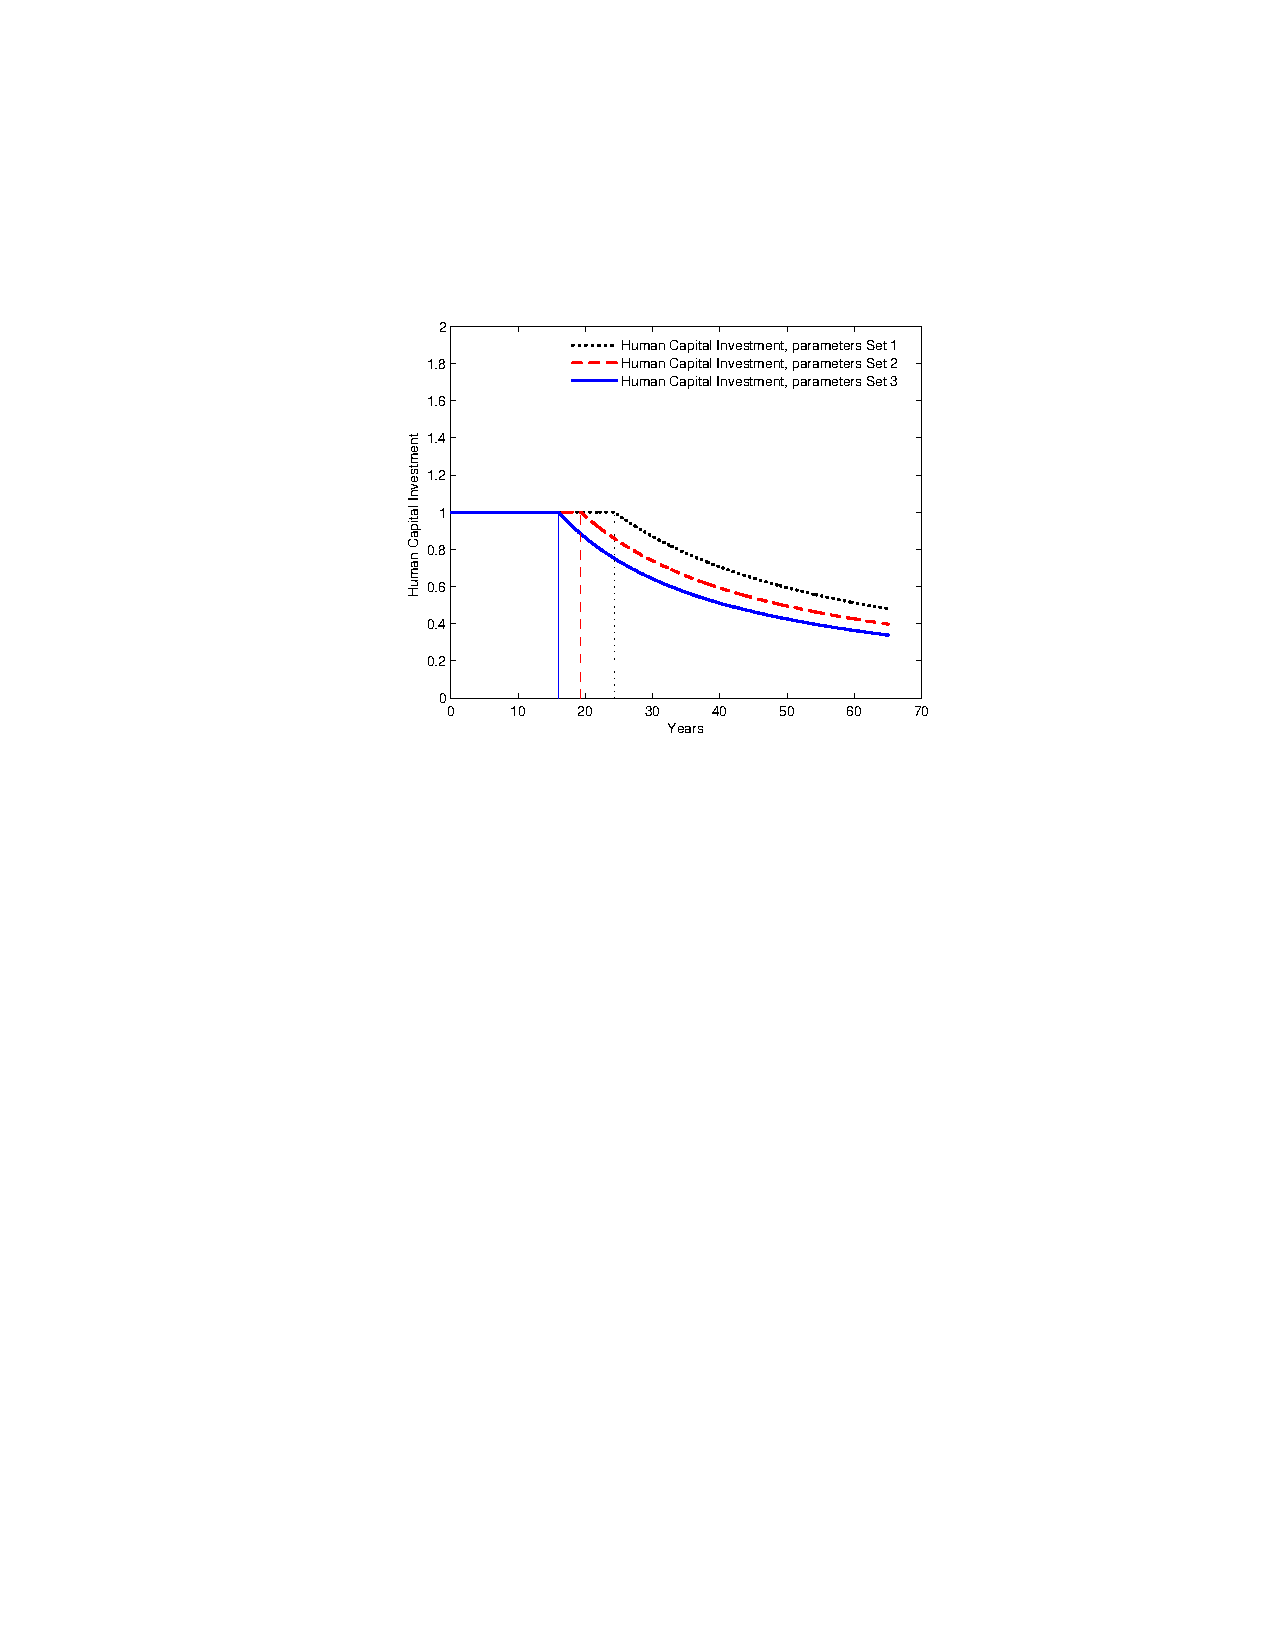
\includegraphics[width=2.2in, height=2.2in]{Figures/fig-hc-earn-series-05.pdf}
        }\\
        \subfigure[Human Capital Stock]{
            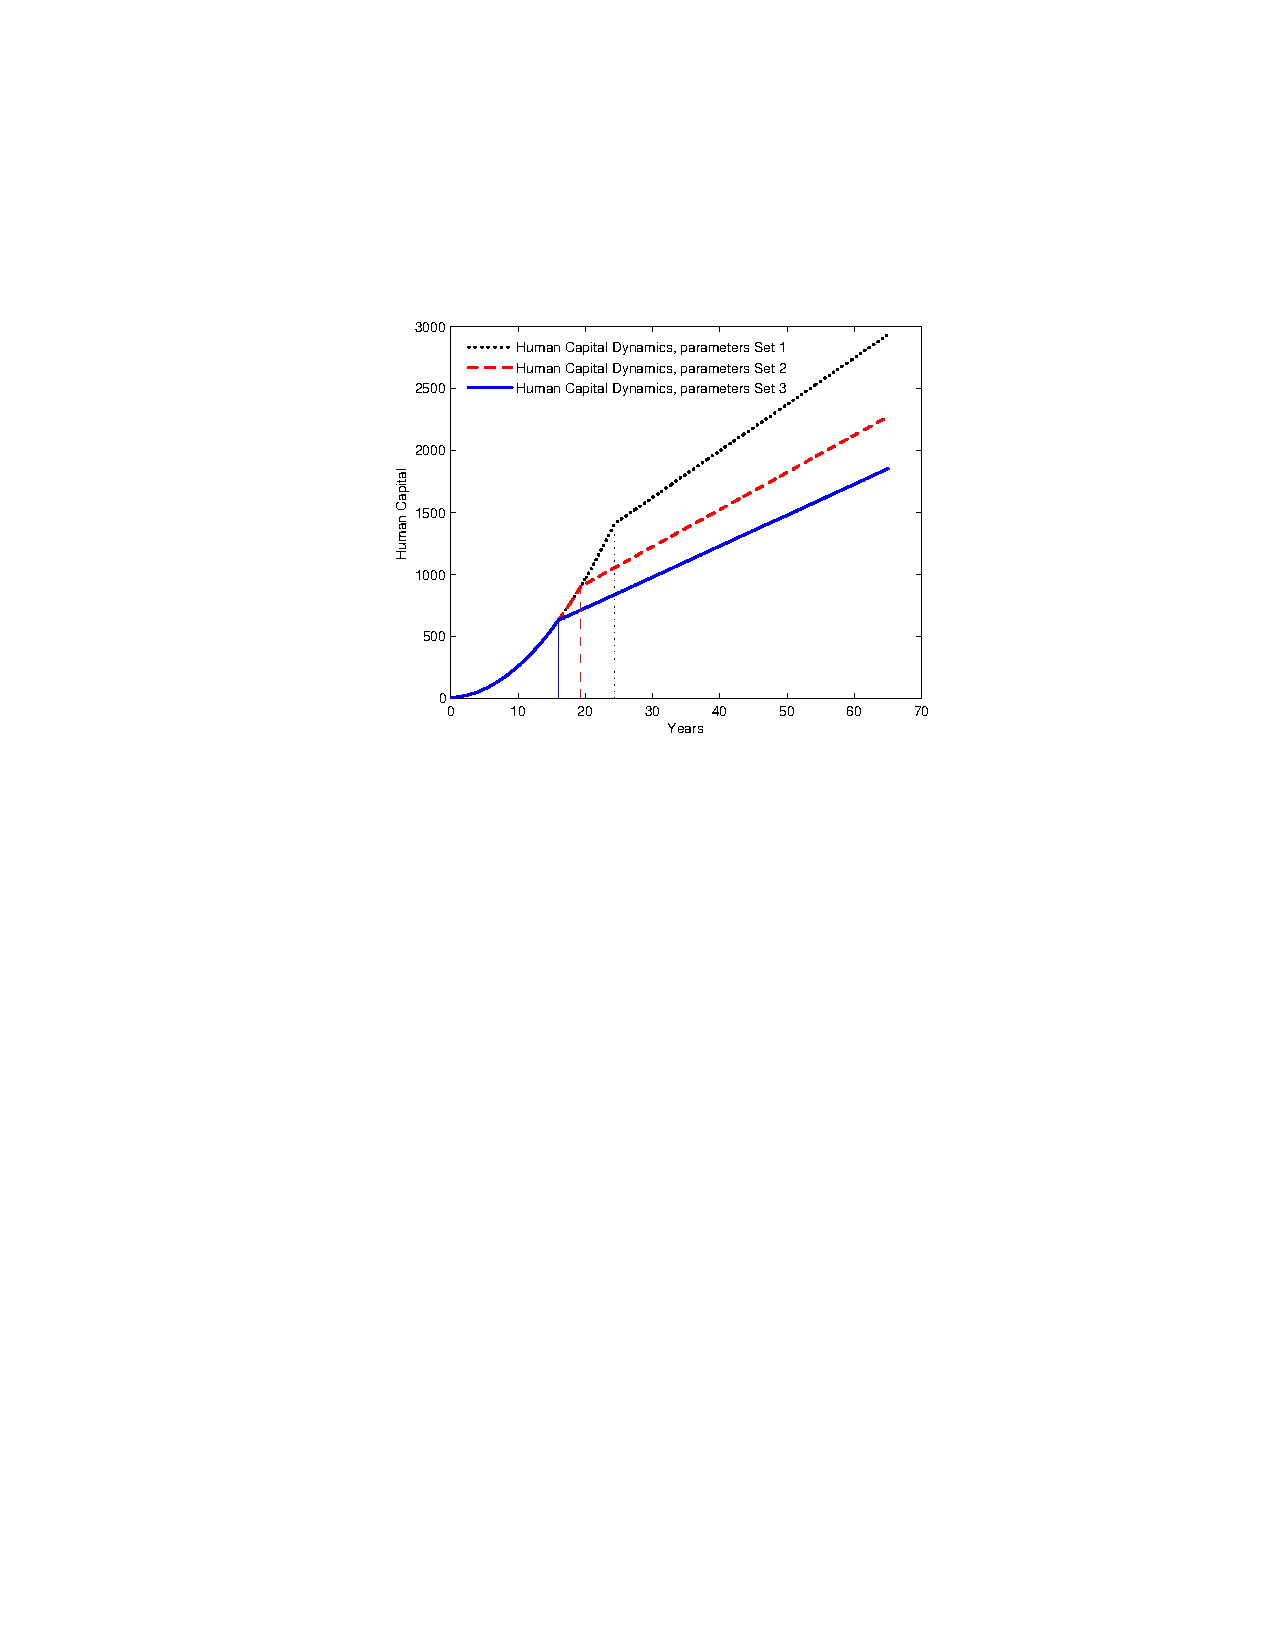
\includegraphics[width=2.2in, height=2.2in]{Figures/fig-hc-earn-series-04.pdf}
        }\\
        \subfigure[Earnings]{%
            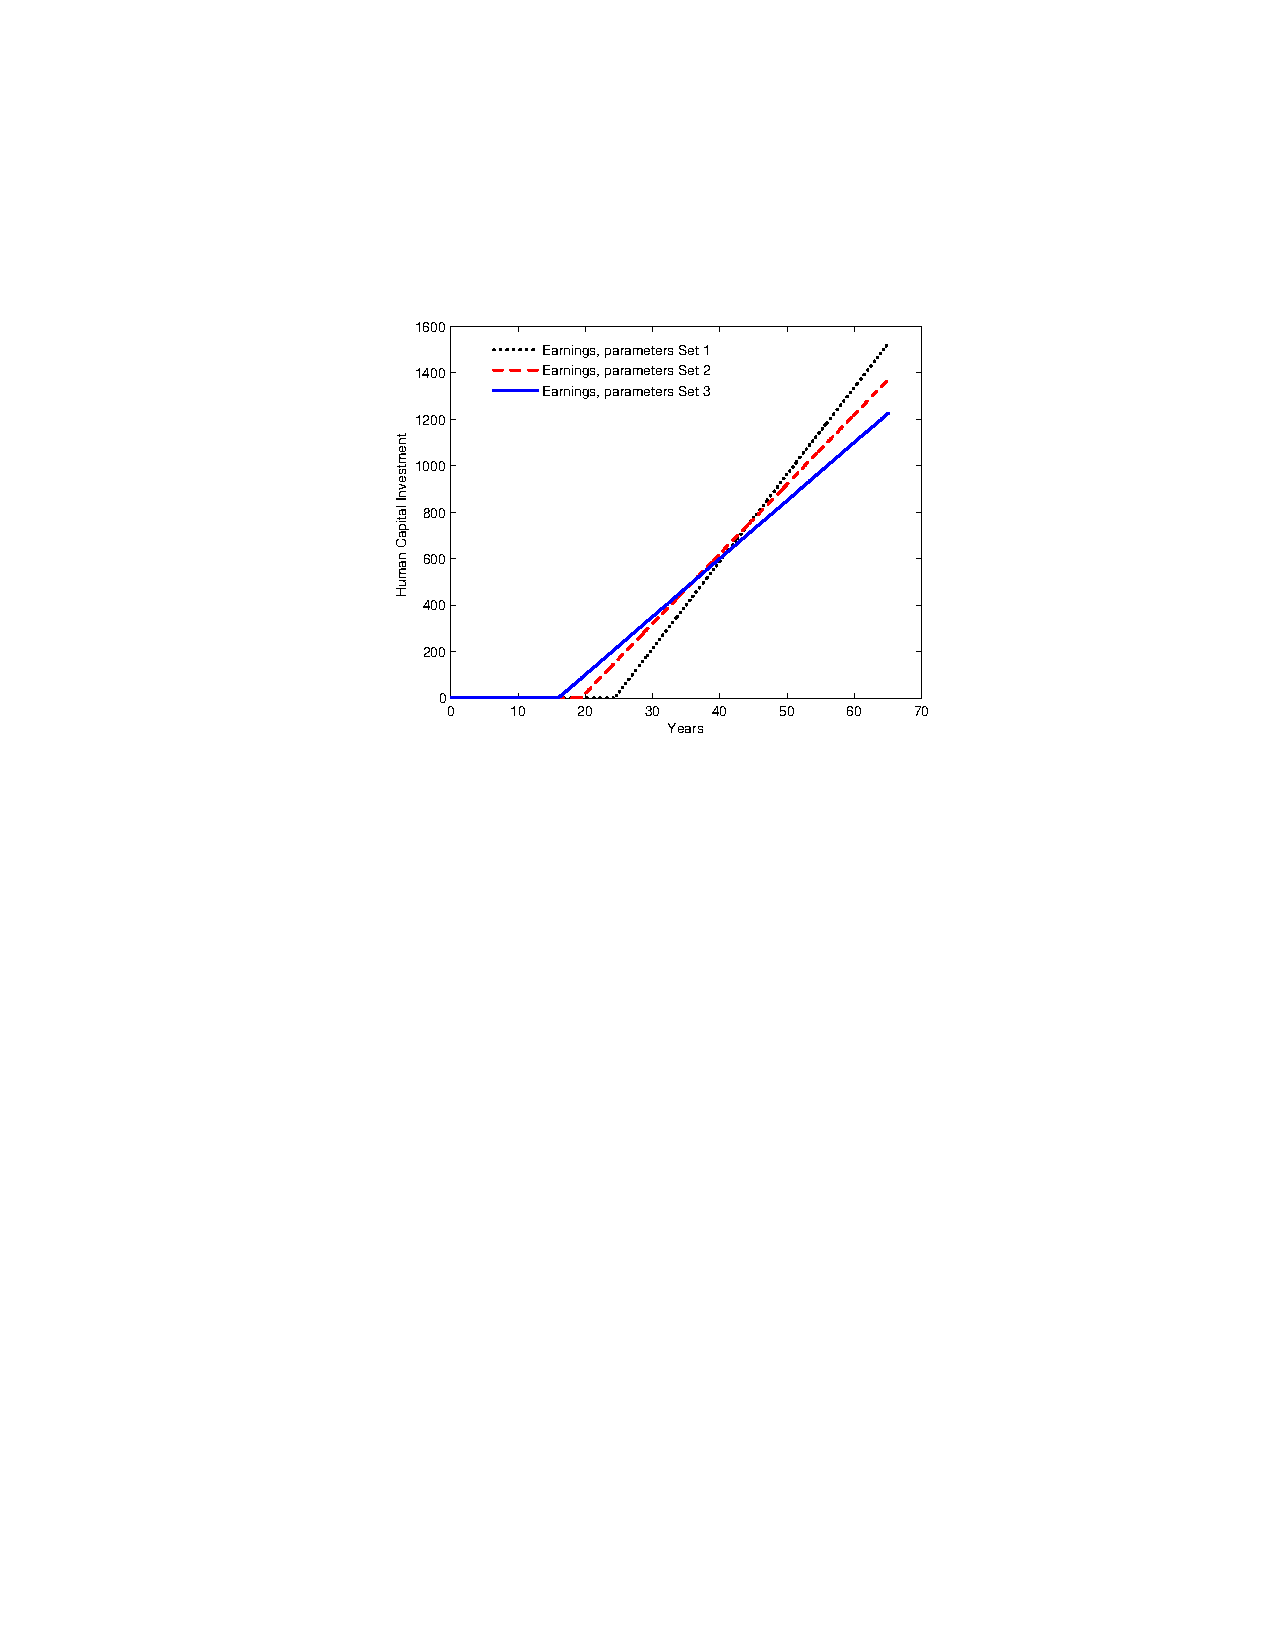
\includegraphics[width=2.2in, height=2.2in]{Figures/fig-hc-earn-series-06.pdf}
        }
\end{figure}

\begin{figure}[H]
\centering
\captionsetup{justification=centering}
   			\caption{Dynamics with Variations in a Production Technology Parameter \\
   			$A = .5$ (dotted); $A = 1.0$ (dashed); $A = 1.5$ (solid) \\
   			for $r = .03, \alpha = .5, H_{0} = 10$ \\  }
        \subfigure[Human Capital Investment]{
            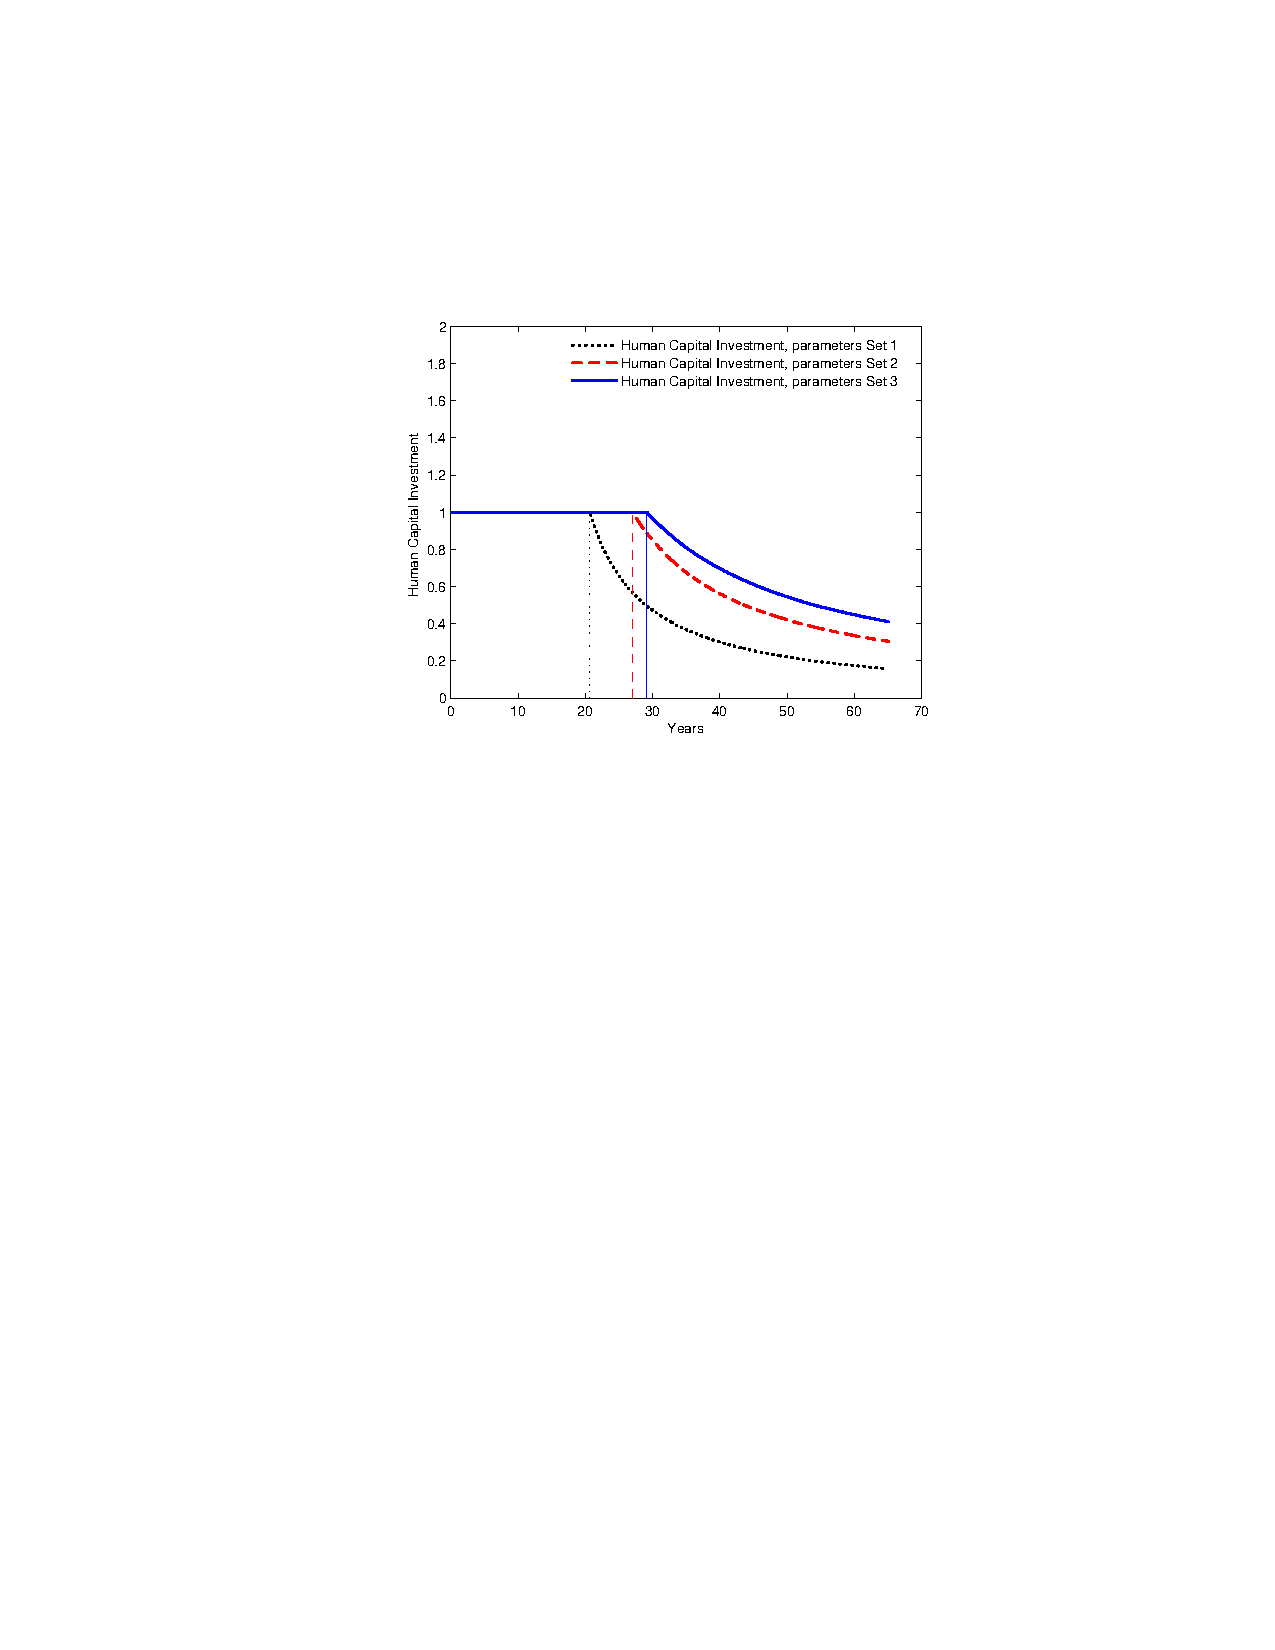
\includegraphics[width=2.2in, height=2.2in]{Figures/fig-hc-earn-series-08.pdf}
        }\\
        \subfigure[Human Capital Stock]{
            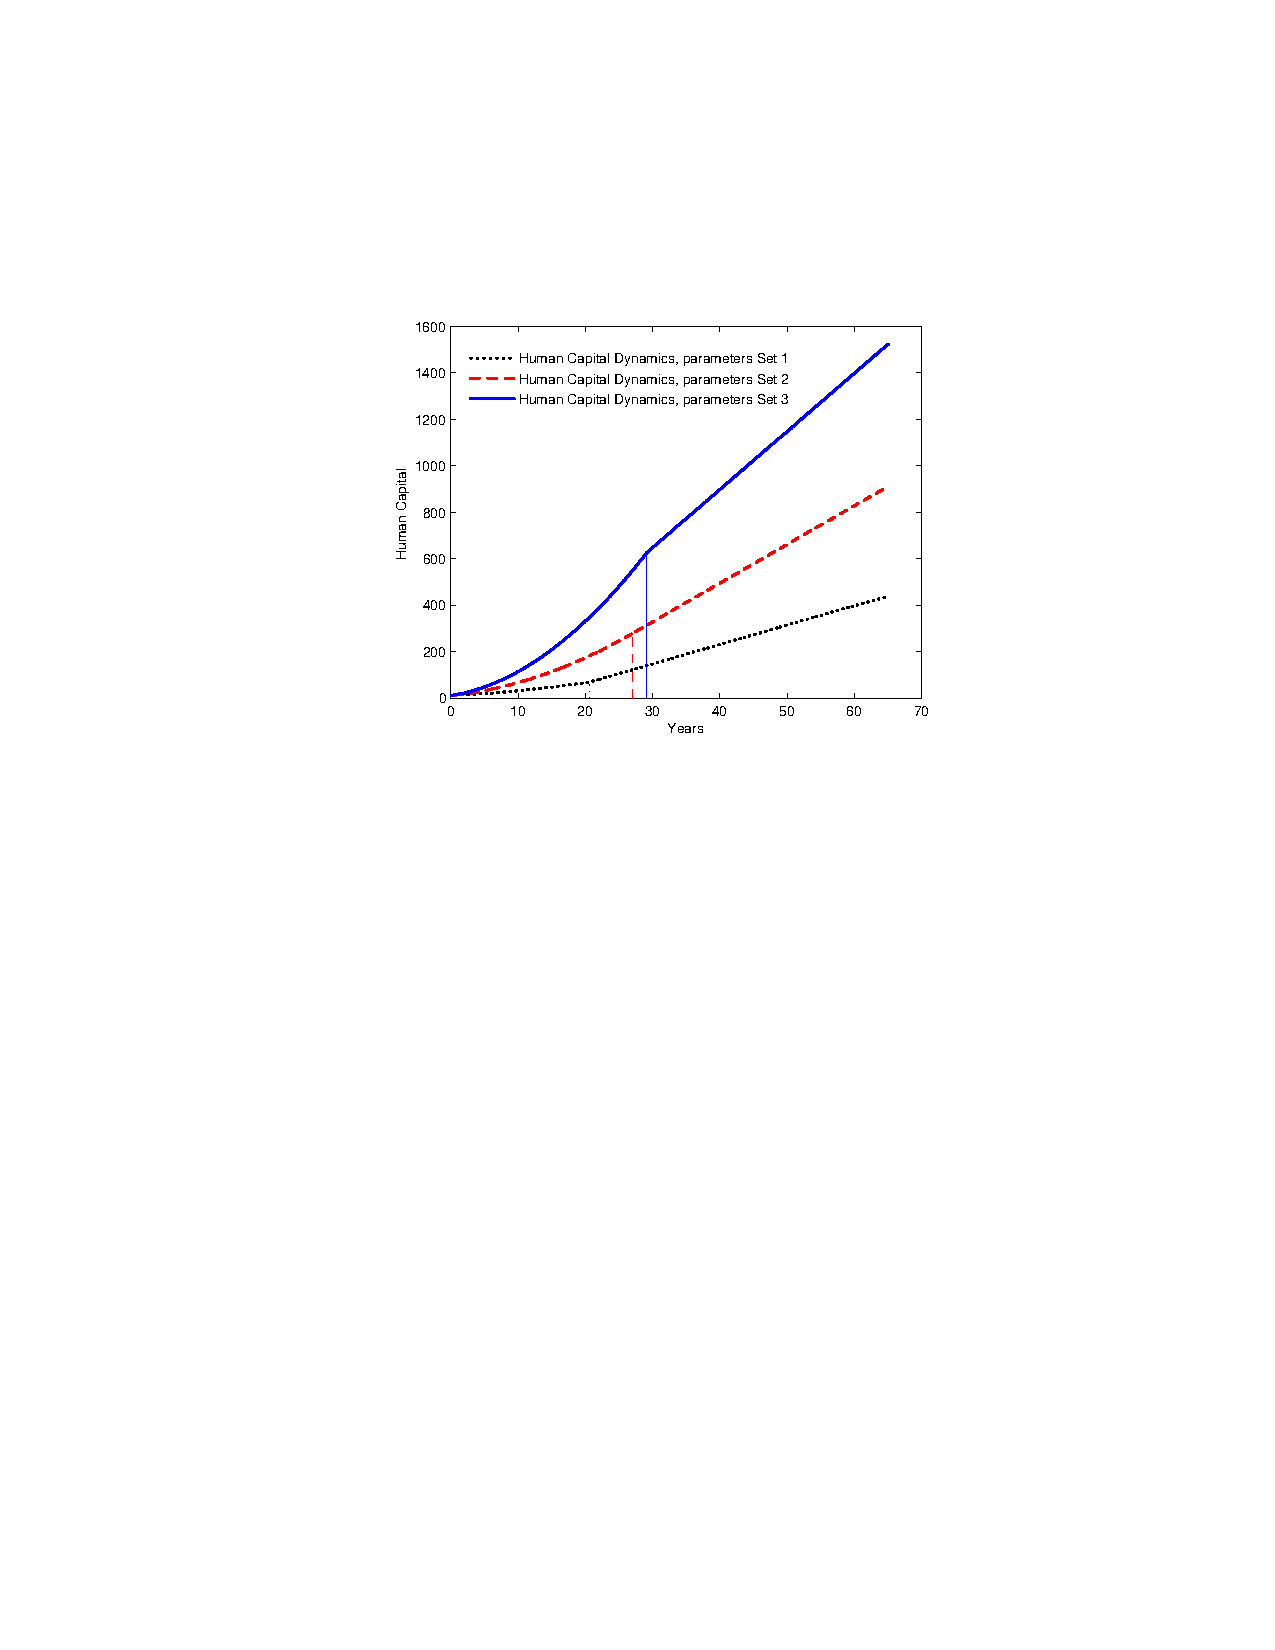
\includegraphics[width=2.2in, height=2.2in]{Figures/fig-hc-earn-series-07.pdf}
        }\\
        \subfigure[Earnings]{%
            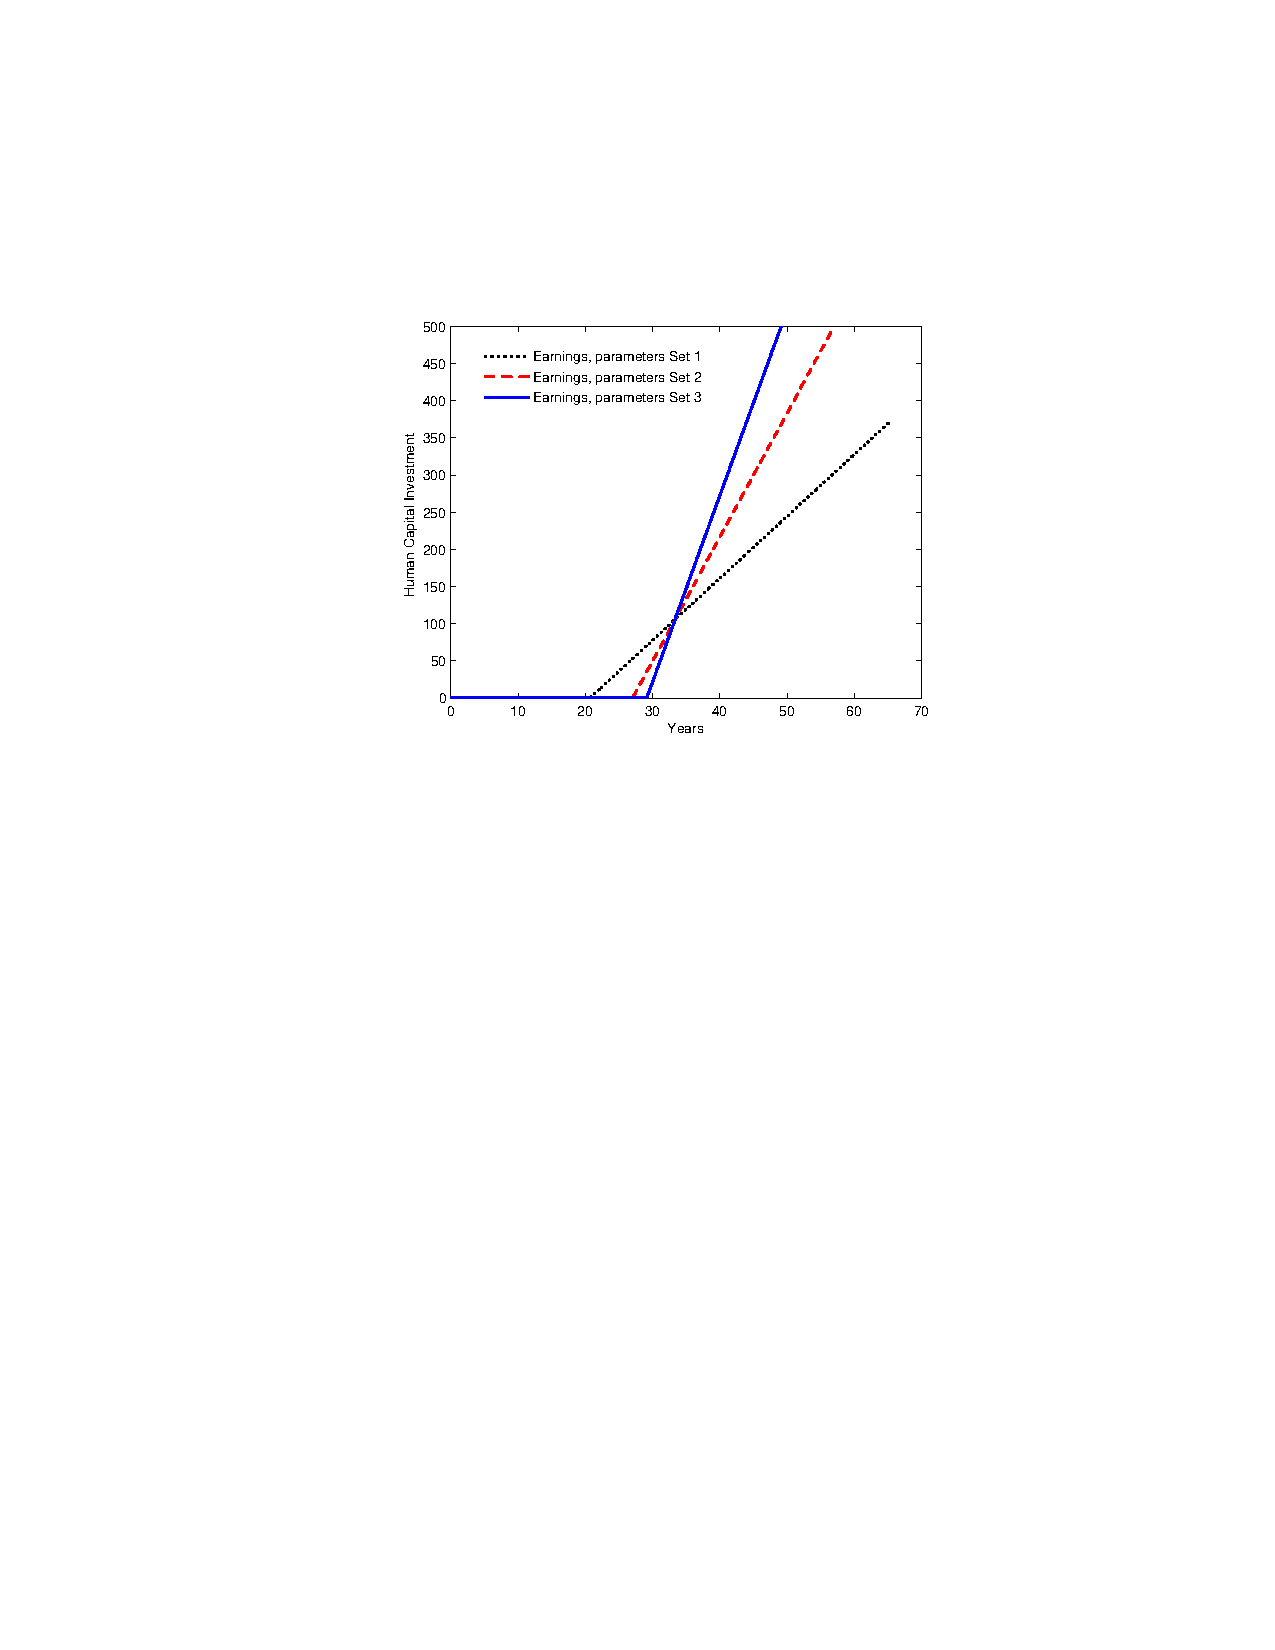
\includegraphics[width=2.2in, height=2.2in]{Figures/fig-hc-earn-series-09.pdf}
        }
\end{figure}

\begin{figure}[H]
    			\centering 
    			\captionsetup{justification=centering}
\caption{Dynamics with Variations in the Initial Level of Human Capital \\ $H_{0} = 10$ (dotted); $H_{0} = 20$ (dashed); $H_{0} = 30$ (solid) \\ for $r = .025, \alpha = .5, A = .6$,}
        \subfigure[Human Capital Investment]{
            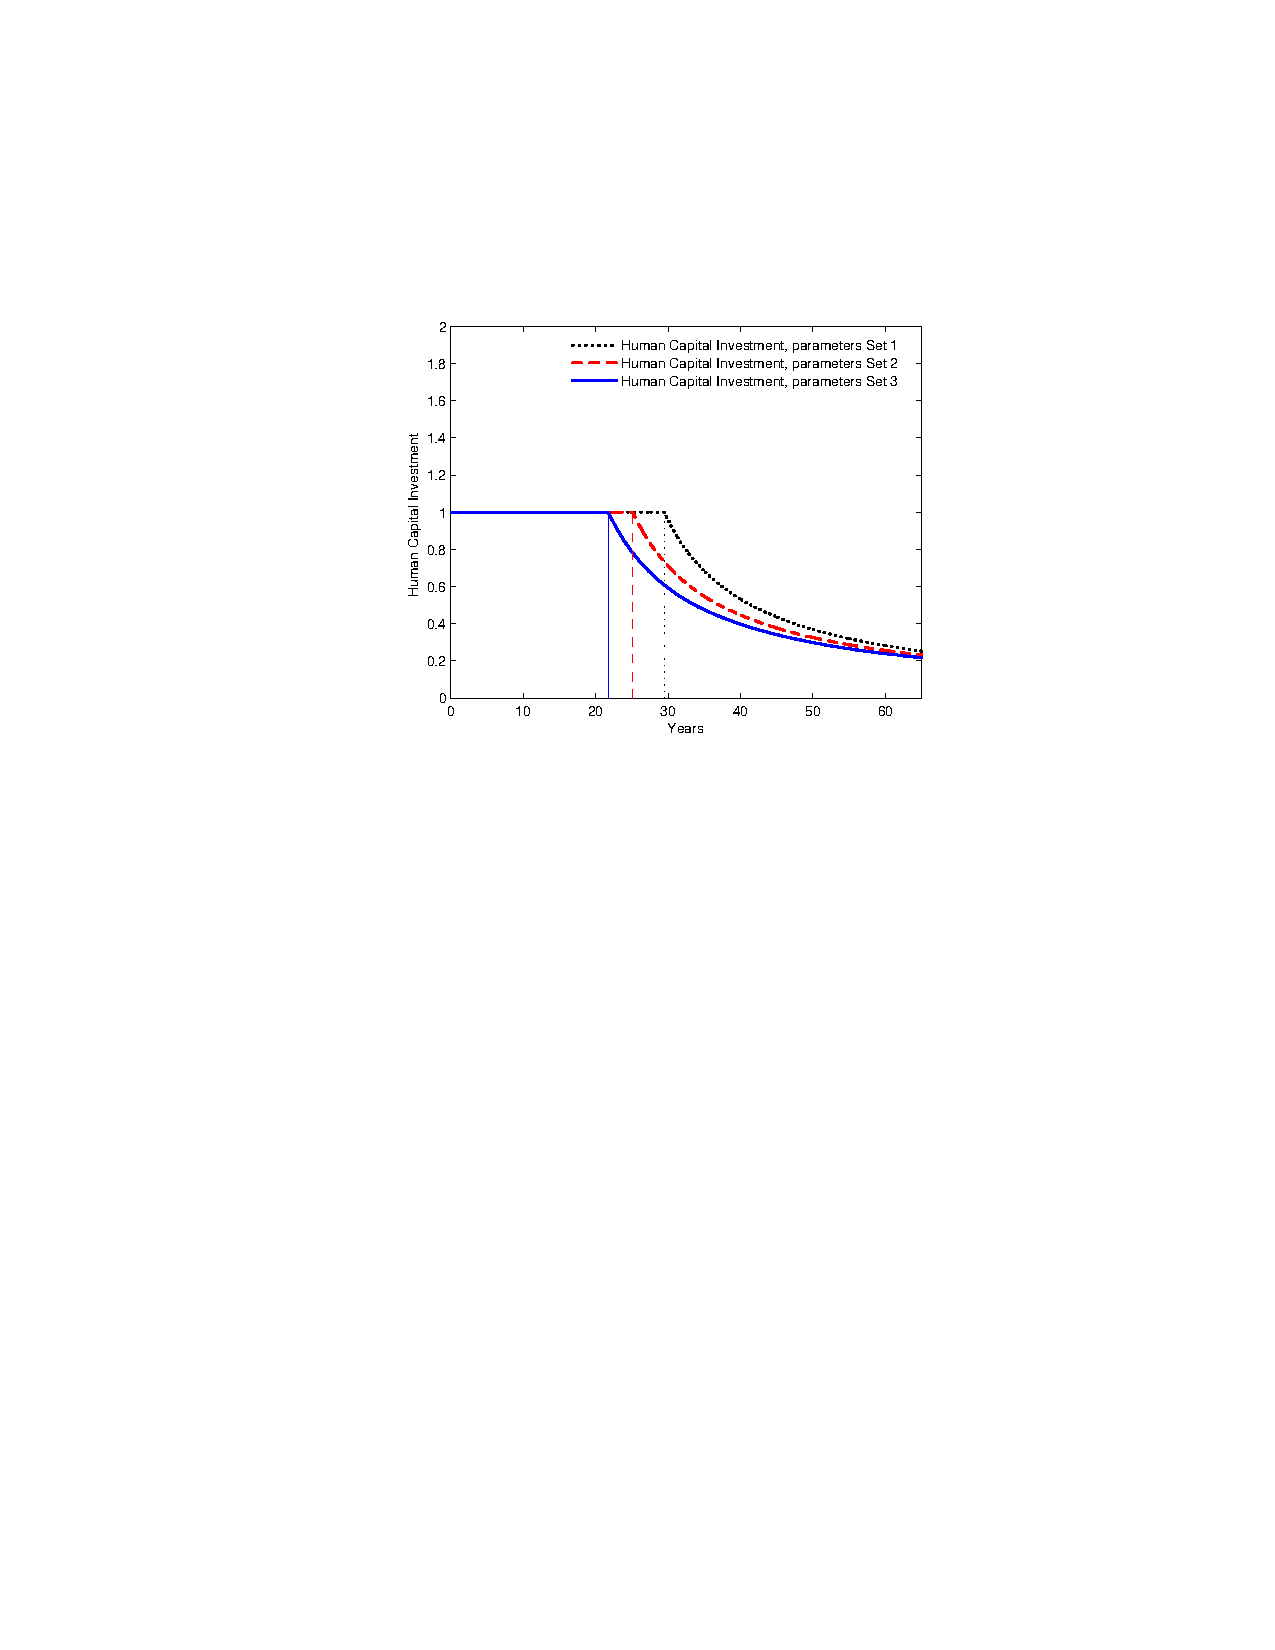
\includegraphics[width=2in, height=2in]{Figures/fig-hc-earn-series-11.pdf}
        }\\
        \subfigure[Human Capital Stock]{
            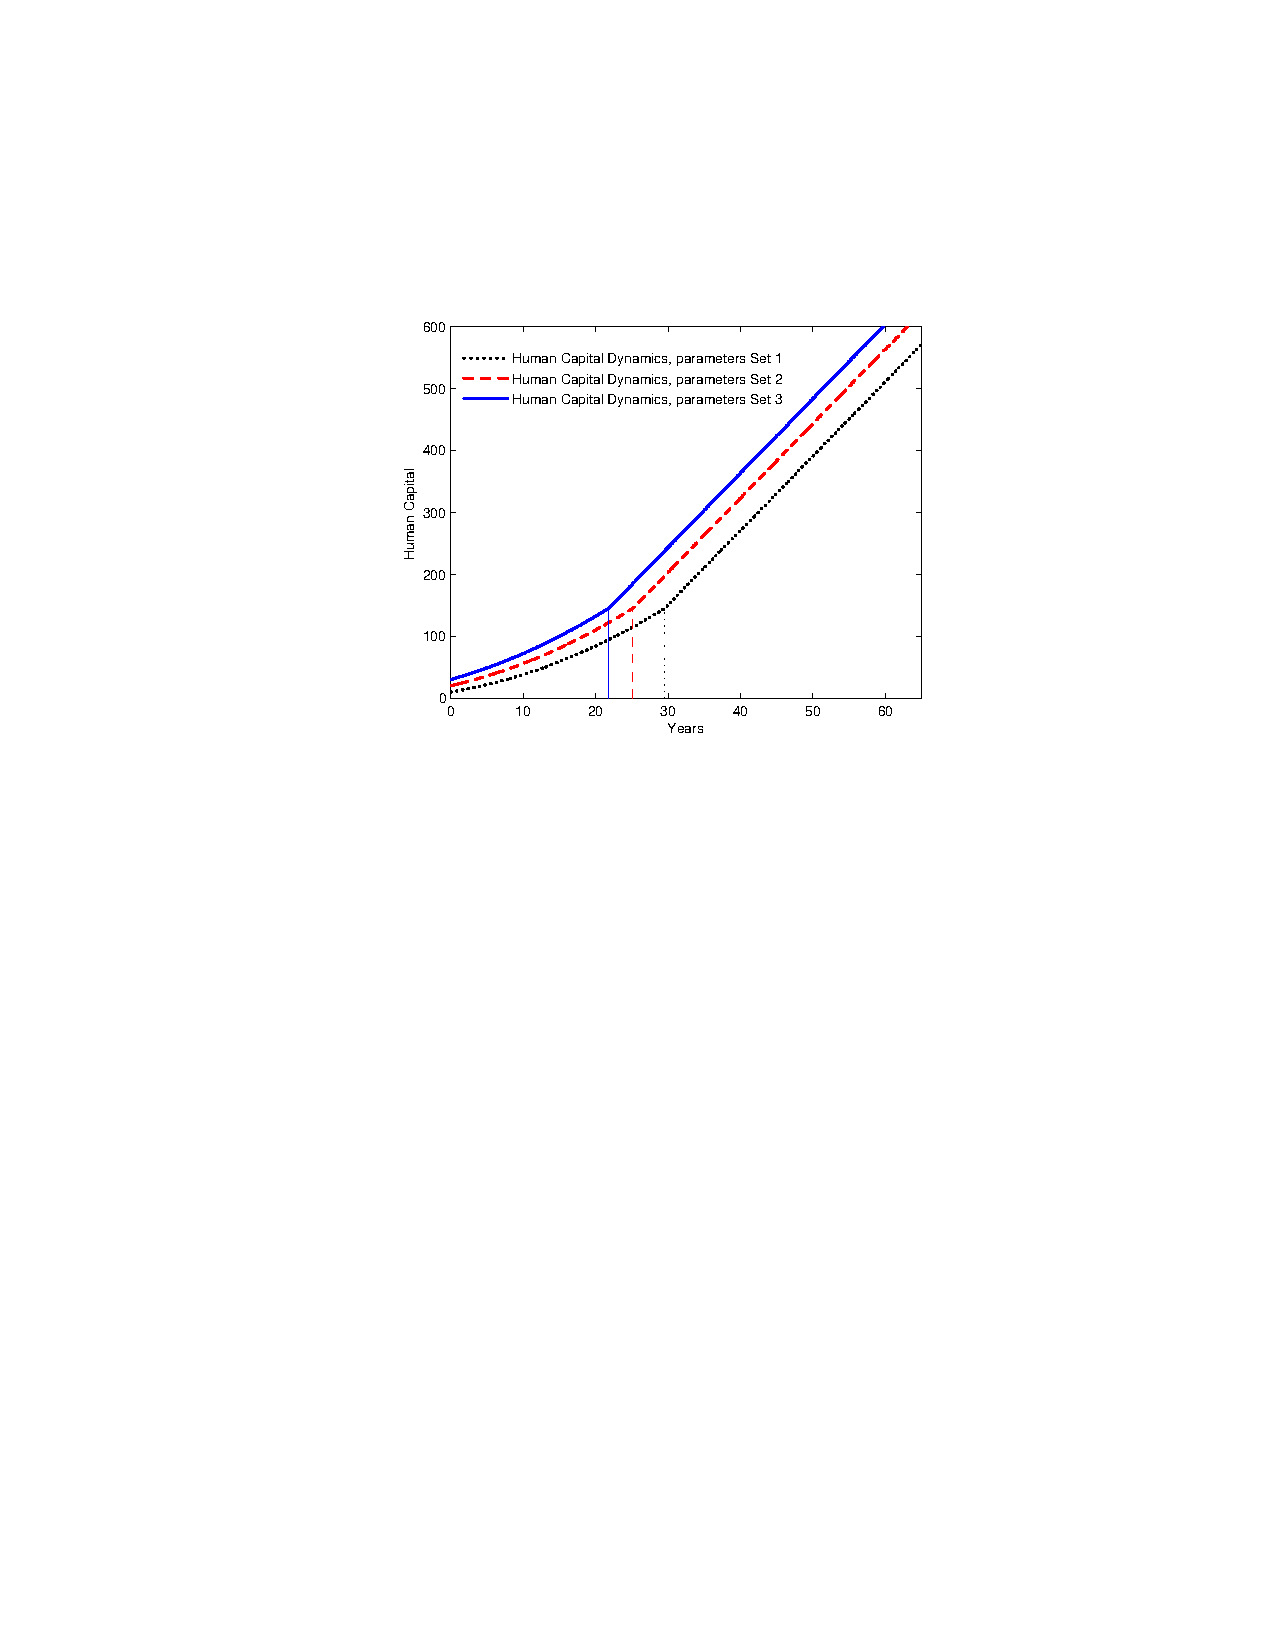
\includegraphics[width=2in, height=2in]{Figures/fig-hc-earn-series-10.pdf}
        }\\
        \subfigure[Earnings]{%
            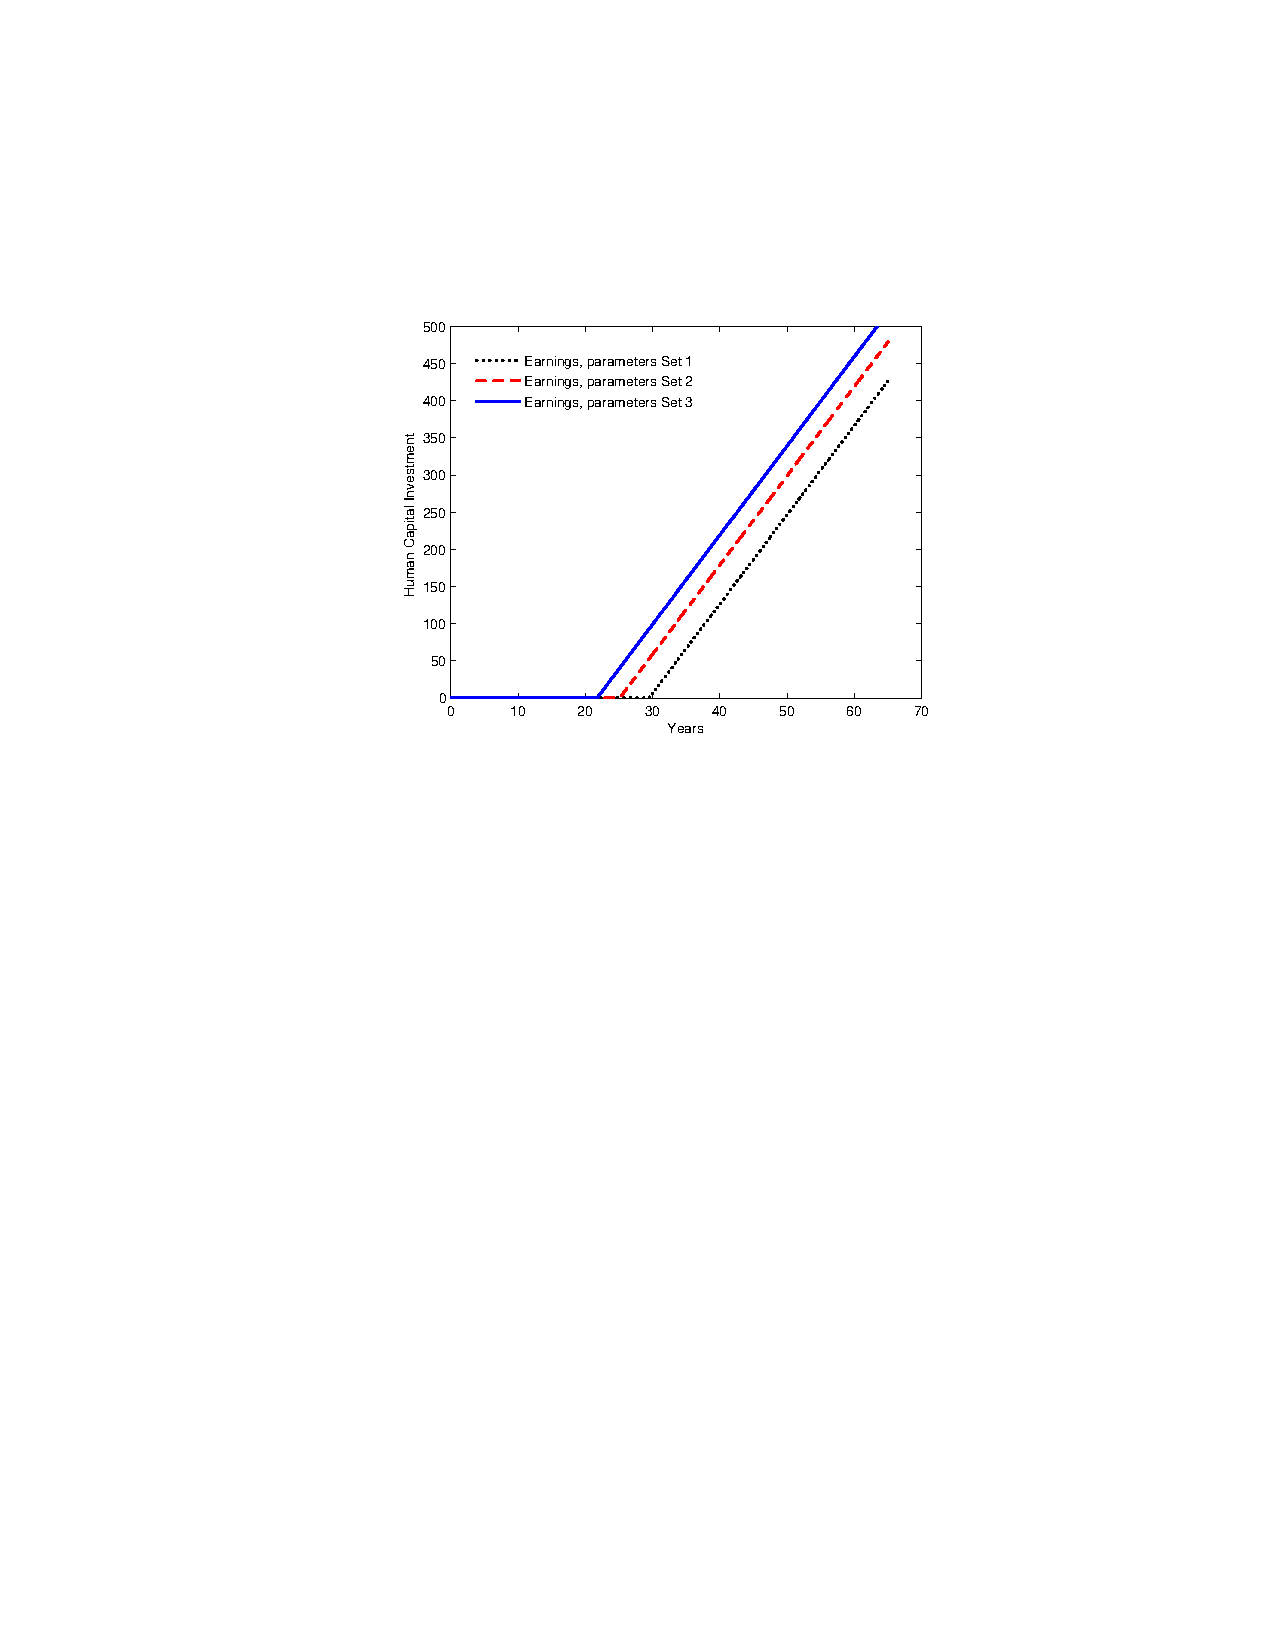
\includegraphics[width=2in, height=2in]{Figures/fig-hc-earn-series-12.pdf}
        }
\end{figure}

\subsection{Rates of Return under the Cobb-Douglas Specification}
We use this model to analyze returns both to schooling and post-schooling. In order to simplify the expressions we let $t \rightarrow  \infty$. Similar implications hold for the finite time horizon problem.

\subsubsection{Return to Schooling}
We call schooling the period of specialization in which the individual devotes his complete human capital stock to produce new human capital. % It's weird that you were using 'her' before and now you suddenly switch to 'his'. Was this on purpose?
To define the return to schooling consider two scenarios: (i) the individual does not invest either in schooling or in post-schooling. Then in each period $t$ she earns $RH_{0}$; (ii) the individual invests in schooling and does not make any post-schooling investments after that. Then in each after-schooling period $\tau$ she earns $R \left[ \frac{\alpha A}{r} \right]^{\frac{1}{1-\alpha}}$. We define the (internal) rate of return of schooling as the discount rate at which the present values of the disposable income streams in the two scenarios are equal.

\begin{definition} (``Internal'' Rate of Return to Schooling)
$\varphi$ is the (internal) rate of return to schooling and solves the equation
\begin{eqnarray}
\int _{t^*} ^{\infty} \exp^{- \varphi t} R \left[ \frac{\alpha A}{r} \right]^{\frac{1}{1-\alpha}} dt &=& \int \limits _{0} ^{\infty} \exp^{- \varphi t} R H_{0} dt \nonumber \\
&\Rightarrow& \nonumber \\
\varphi &=& \frac{\ln \left[ \frac{\alpha A}{r} \right]^{\frac{1}{1 - \alpha}} - \ln H_{0}}{-\frac{H_0^{1-\alpha}}{A(1-\alpha)}+\frac{\alpha}{1-\alpha} \frac{1}{r}}.
\end{eqnarray}
\end{definition}

\subsubsection{Return to Post-schooling}
Let $E(\tau)^{NPS}$ and $E(\tau)^{PS}$ denote earnings with and without post-schooling investment, respectively. By \eqref{eq:earnsall} we can write
\begin{eqnarray}
E(\tau)^{NPS} &=& R H(t^*) \\ \nonumber
&=& R \left( \frac{\alpha A}{r} \right)^{\frac{1}{1 - \alpha}} \\ \nonumber
E(\tau)^{PS} &=& R A \left[ \frac{\alpha A}{r} \right]^{\frac{\alpha}{1-\alpha}} \tau
\end{eqnarray}

\noindent so that the increment in earnings due to post-schooling at $\tau$ is
\begin{eqnarray}
\Delta^{E(\tau)} \equiv E(\tau)^{PS} - E(\tau)^{NPS}.
\end{eqnarray}

\indent We can interpret $\Delta^{E(\tau)}$ as ``returns less costs'' from post-schooling, with $E(\tau)^{NPS}$ as the costs (i.e. foregone earnings) of post-schooling investments. Then, we define the (internal) rate of return to post-schooling as follows.

\begin{definition} (``Internal'' Rate of Return to Post-schooling)
$\phi$ is the (internal) rate of return to schooling and solves the equation
\begin{equation}
\int \limits _{0} ^{\infty} \exp^{- \phi \tau} \left[ R A \left[ \frac{\alpha A}{r} \right]^{\frac{\alpha}{1-\alpha}} \tau - R \left( \frac{\alpha A}{r} \right)^{\frac{1}{1 - \alpha}} \right] d \tau = 0 \label{eq:postreturn}
\end{equation}
\noindent Using the Laplace transform, \eqref{eq:postreturn} implies
\begin{eqnarray}
\frac{1}{\phi^2} RA \left[ \frac{\alpha A}{r} \right]^{\frac{\alpha}{1-\alpha}} - \frac{R}{\phi} A \left[ \frac{\alpha A}{r} \right]^{\frac{1}{1-\alpha}} &=& 0 \nonumber \\
&\Rightarrow& \nonumber \\
\phi &=& \frac{r}{\alpha}.
\end{eqnarray}
\end{definition}

\indent The (internal) rate of return to post-schooling investment is a decreasing function of $\alpha$. Recall that the internal rate of return of post-schooling measures the desirability of the investment opportunity, and with a higher $\alpha$, individuals' levels of human capital are relatively high, even without any post-schooling investment. Therefore, the relative differences (measured by the ratios) between the amount of disposable earnings in cases with and without investment are smaller. Therefore, investment in post-schooling is less desirable for more productive individuals. In addition, relatively patient individuals (who have relatively low $r$) require a smaller discount rate $\phi$ to equalize the scenarios with and without post-schooling investment.

\subsection{Earnings Growth and Patience in Finite Horizon}
In this section we want to ask, in the same framework, how earnings growth depend on what defines relative patience in this model, the discount rate $r$. To do that, we investigate $\frac{\partial \dot{E(\tau)}}{\partial r}$.

\begin{claim} \label{claim:moreconcwithighr}
Assume that $1 - \frac{F'(\cdot) F'''(\cdot)}{{F''}^2} < 0$ (recall from Claim \ref{claim:concearnnodep} that this is a sufficient condition for $\ddot{E(t)}<0$ in the current context). Then, $\frac{\partial \dot{E(\tau)}}{\partial r} < 0$.
\end{claim} 

\begin{proof}
Without loss of generality, assume that R =1 and note that\\
\begin{equation}
\frac{\partial \dot{E(\tau)} }{\partial r} = F'(\cdot) \frac{\partial IH}{\partial r} - \frac{\partial}{\partial r} \dot{IH}. \label{eq:earnpartialr}
\end{equation}

\noindent From \eqref{eq:newfocs} we know that the first order condition of the agent's problem is
\begin{equation}
g(t) F'(\cdot) = 1
\end{equation}

\noindent which by the implicit function theorem yields
\begin{eqnarray}
\frac{\partial IH}{\partial r} &=& \frac{\frac{\partial g(t)}{\partial r} F'(\cdot)}{2 g(t) F''(\cdot)} \nonumber \\ 
&<& 0
\end{eqnarray}

\noindent where the inequality follows from strict concavity of $F(\cdot)$ and  $\ g(t) > 0, \frac{\partial g(t)}{ \partial r} <0$ (see \eqref{eq:partialgr}). Thus, the first term in \eqref{eq:earnpartialr} is negative. If we show that the second term is negative then we can sign \eqref{eq:earnpartialr} and give meaning to these results. In order to do so we need $\frac{\partial \dot{IH}}{\partial r} > 0$. From \eqref{eq:itdot} note that 
\begin{equation}
\frac{\partial \dot{IH}}{\partial r} = -\frac{\dot{g}}{g} \left[ 1 - \frac{F'(\cdot)F'''(\cdot)}{{F''(\cdot)}^2}\right] \frac{\partial IH}{\partial r} + \frac{F'(\cdot)}{F''(\cdot)}\frac{\partial}{\partial r} \left[ - \frac{\dot{g}}{g} \right] \label{eq:ihdotr}
\end{equation}

\indent We know from $1 - \frac{F'(\cdot) F'''(\cdot)}{{F''}^2} < 0$ and $\dot{g}, \frac{\partial IH}{\partial r} < 0$ that the first term in \eqref{eq:ihdotr} is positive. To sign the second term note that $\dot{g} = rg - 1, - \frac{\dot{g}}{g} = \frac{1}{g} - r$. Then,
\begin{equation}
\frac{\partial}{\partial r} \left[ - \frac{\dot{g}}{g} \right] = - \frac{1}{g^2} \frac{\partial g}{\partial r} - 1. \label{eq:dotgg}
\end{equation}

\indent To sign \eqref{eq:dotgg} note that
\begin{eqnarray}
\frac{\partial g}{\partial r} &=& \frac{\exp^{r(t-T)} \left( 1 - r(t - T) \right) - 1 }{r^2} \nonumber \\
&<& 0 \label{eq:partialgr}
\end{eqnarray}

\noindent and

\begin{eqnarray}
- \frac{\partial g }{g^2 \partial r} - 1 &=& \frac{1}{r^2g^2} \exp^{r(t-T)} \left( 1 + r(t - T) - \exp^{r(t-T)} \right). \nonumber \\
&<& 0
\end{eqnarray}

\noindent which implies that $\frac{\partial \dot{E}}{\partial r} < 0$. 
\end{proof}

\indent The graphical representation of Claim~\ref{claim:moreconcwithighr} is in Figure~\ref{fig:earnprofr}. It implies that the earnings function is relatively ``less concave'' for relatively impatient individuals (relatively high $r$). This is a consequence of their investment decisions: they spend less time in the schooling period and accumulate less human capital.

\begin{center}
\begin{figure}[H]
\caption{Earnings Profiles in Finite Horizon for Different Values of $r$ } \label{fig:earnprofr}
\centering
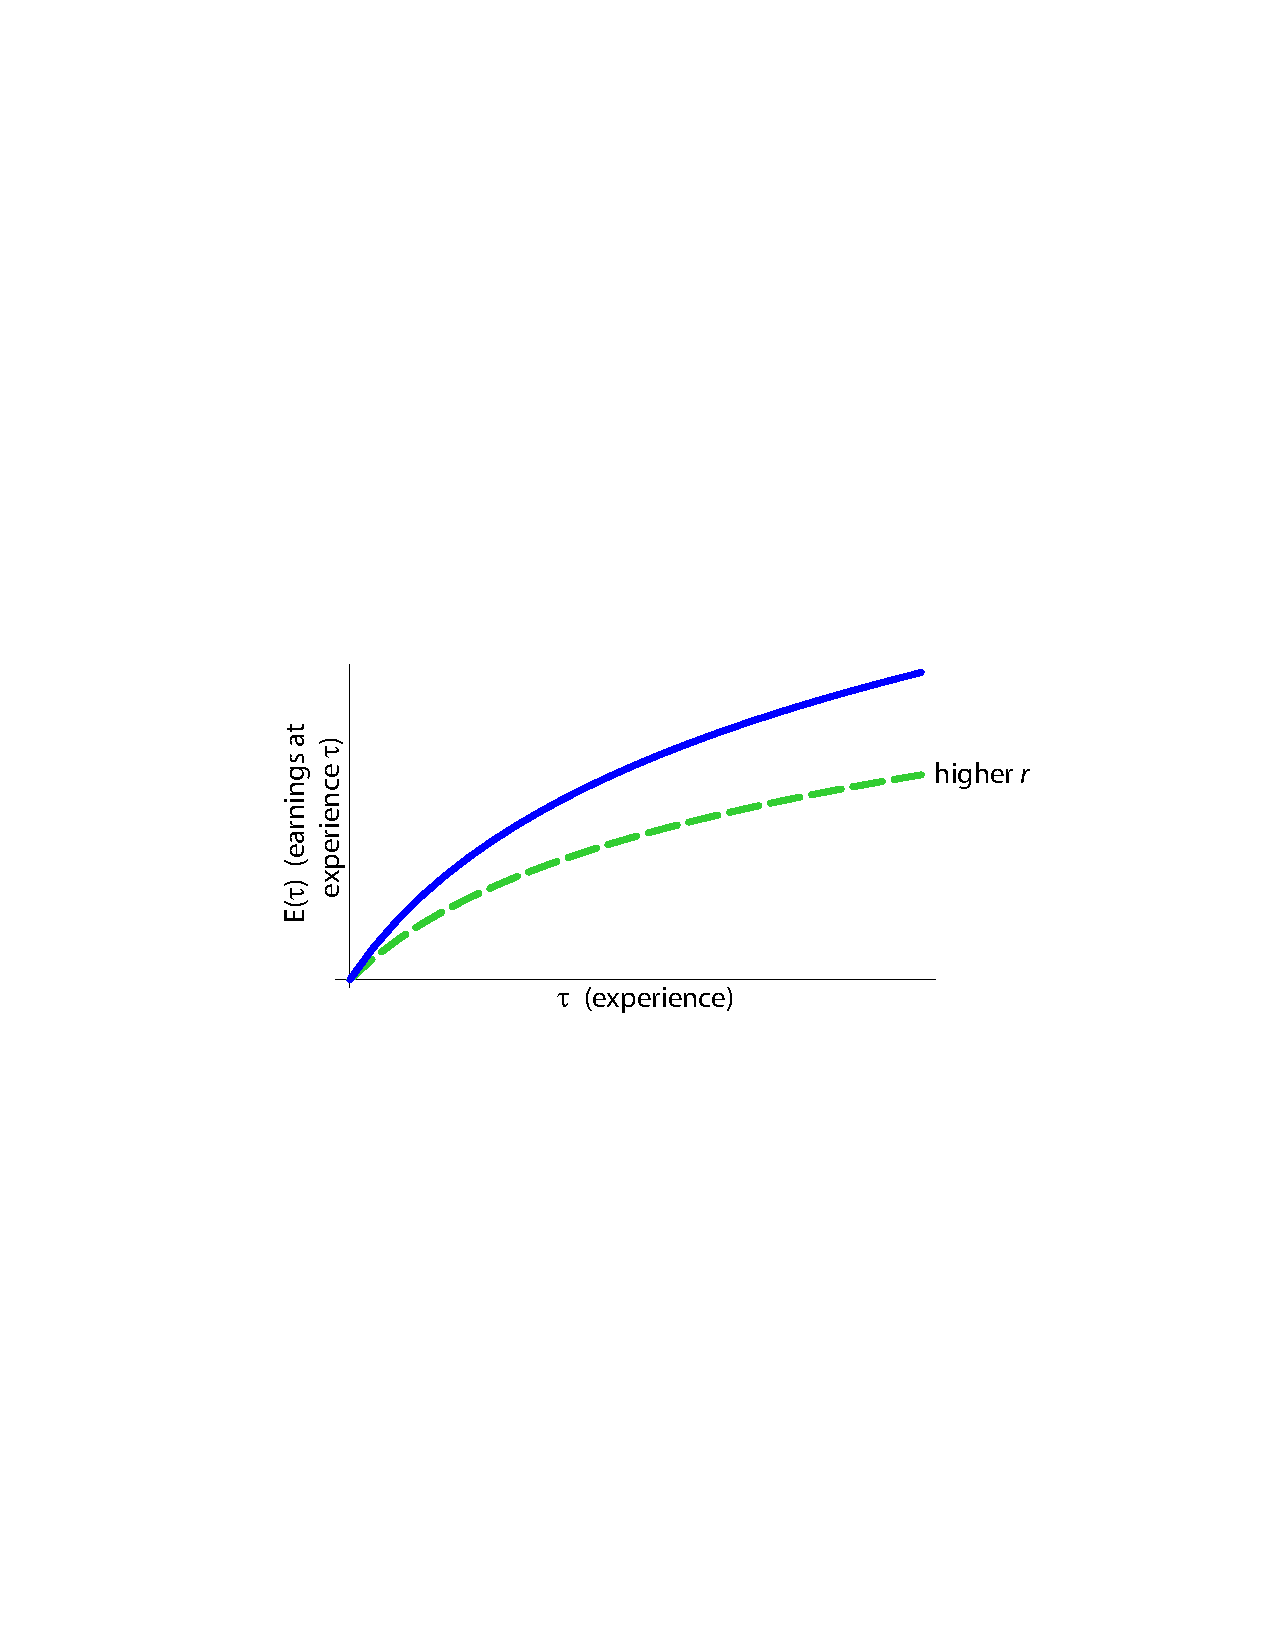
\includegraphics[width=3.5in, height=1.5in]{Figures/fig-earnings-growth.pdf}
\floatfoot{\begin{small}
\end{small}}
\end{figure}
\end{center}

\section{The Haley-Rosen Specification: Finite Horizon and the Autoregression Form}
We analyze the finite horizon case under the specification that \citet{haley1976estimation} and \citet{rosen1976theory} use. Specifically, we assume that $\dot{H} = A \left( IH \right)^{\alpha}, \alpha = \frac{1}{2}, \sigma = 0$ and the exact same setting as in Section \ref{section:baseline}. Actually, in Section \ref{section:baseline} we rely on an infinite horizon to derive a set of closed form solutions to the individual's problem. In this section we relax the infinite horizon assumption and rely on the assumption $\alpha = \frac{1}{2}$ to gain tractabiliy.\\
\indent We focus on the dynamics of post-schooling earnings because one of the less credible consequences of the infinite horizon is the linearity of earnings on experience. From \eqref{equation:postearnings} we can write
\begin{eqnarray}
E(\tau) &=& RH(t^*) + R \int \limits _{0} ^{\tau} A \left[\frac{1}{2} \frac{g(t^* + l)A}{R} \right]dl - R \left[\frac{1}{2} \frac{g(t^* + \tau)A}{R} \right]^{2} \nonumber \\
&\Rightarrow& \nonumber \\
\dot{E(\tau)} &=& \frac{g (t^* + \tau)A^2}{2R}\left( 2R -rg (t^* + \tau) \right) \nonumber \\
&\Rightarrow& \nonumber \\
\ddot{E(\tau)} &=& -\frac{A^2}{R}\dot{g(t^* + \tau)}^2 \label{eq:earnalpha2}
\end{eqnarray}
where the second and third equalities use \eqref{eq:grossdep}. Combining \eqref{eq:grossdep} and \eqref{eq:earnalpha2} we obtain a second order ODE with constant coefficients:
\begin{equation}
\ddot{E(\tau)} = 2r \dot{E(\tau)} - A^2 R \label{eq:earndifferential}
\end{equation} 

\noindent where the natural initial and terminal conditions that we impose are $E(0)=0$ and $\dot{E(T)} = 0$ and then we guess and verify that the general solution to \eqref{eq:earndifferential} is the following. %you 'guess' and then verify?? what does that even mean. You shouldn't say you're 'guessing' anything.
\begin{equation}
E(\tau) = c_{0} + c_{1}\exp^{-2r \tau} + c_{2} \tau
\end{equation}

\indent So $E(0)=0$ implies $c_{1} + c_{0} = 0$ and $\dot{E(T)} = 0$ implies $2rc_1 \exp^{2rT}  + c_{2} = 0$. Together with \eqref{eq:earndifferential}, we can solve for $c_0 = \frac{A^2 R}{4r^2 \exp^{2rT}}$, $c_1 = -c_0$, and $c_2 = \frac{A^2 R}{2r}$. Therefore, 

\begin{equation}
E(\tau) = \frac{A^2 R}{4r^2} \exp^{-2r T} \left( 1 - \exp^{2r \tau} \right) + \frac{A^2 R}{2r} \tau. \label{eq:earningspostalpha12}
\end{equation}

\begin{center}
\begin{figure}[H]
\caption{Post-school Earnings in the Haley-Rosen Specification}
\centering
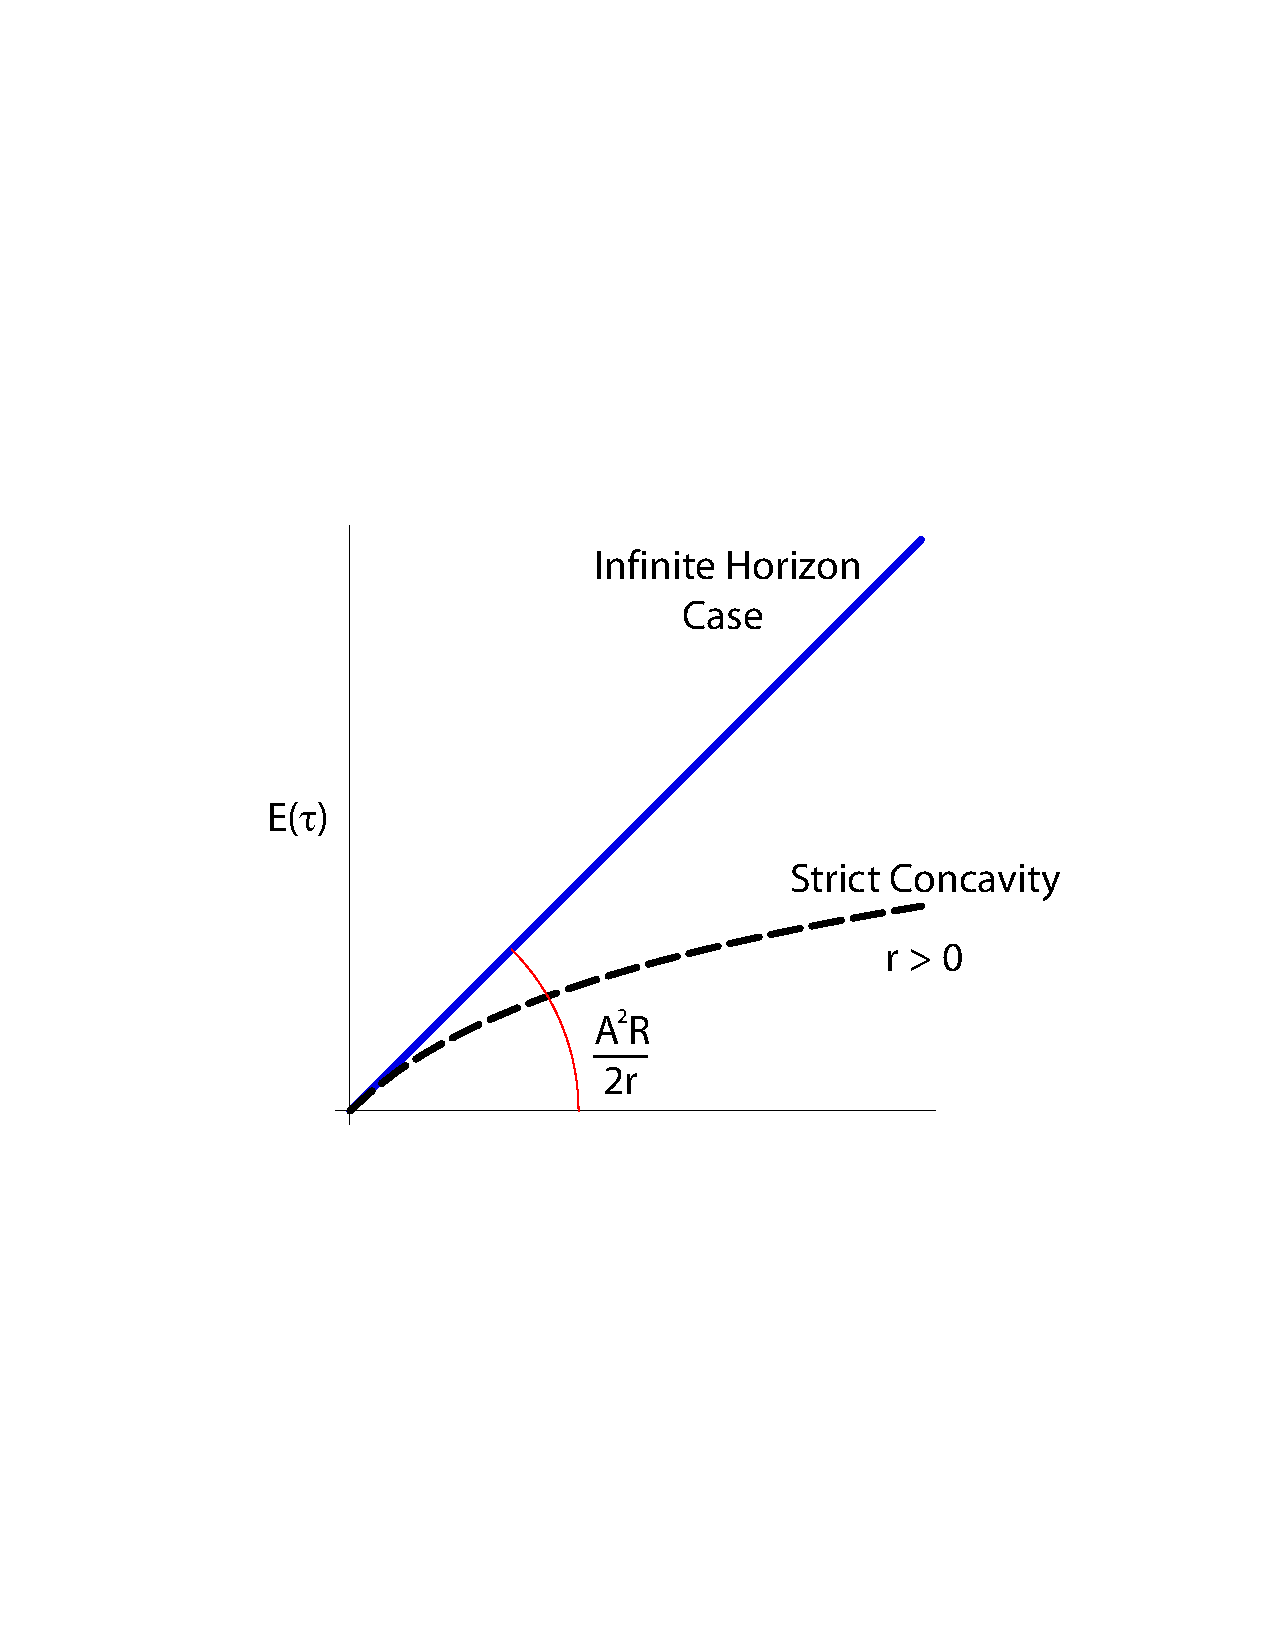
\includegraphics[width=3.5in, height=1.5in]{Figures/fig-finite-horiz.pdf}
\floatfoot{\begin{small}
Note:
\end{small}}
\end{figure}
\end{center}

\indent From \eqref{eq:earnalpha2}, we know that in the finite horizon case, the earnings function is strictly concave unless $t=T$. The intuition behind the linearity of the earnings function in the infinite horizon case is provided in Section \ref{section:specialization}. In contrast with the infinite case, the return to investment is decreasing over time as the agent is approaching the final period of the time horizon, which implies that $I(t)H(t)$ is decreasing overtime. Thus the stock of human capital is increasing at a decreasing rate, which leads to the concavity of earnings dynamics. 

\subsection{The Autoregression}
From \eqref{eq:earningspostalpha12} it is possible to write
\begin{equation}
E(\tau + 1) - E(\tau) =  \frac{A^2 R}{2r}+ \frac{A^2 R}{4r^2} \exp^{-2rT} \left( \exp^{2r\tau} - \exp^{2r(\tau+1)} \right) 
\end{equation}

\noindent which implies that

\begin{equation}
z(\tau + 1) = \exp^{2r} z(\tau) + \frac{A^2 R}{2r} \left( 1 - \exp^{2r} \right) \label{eq:growthalpha12}
\end{equation}

\noindent where $z(\tau) \equiv E(\tau + 1) - E(\tau)$ and we can analyze the growth dynamics of earnings. Consider a visual representation of \eqref{eq:growthalpha12}

\begin{center}
\begin{figure}[H]
\caption{Earnings Growth in the Haley-Rosen Representation}
\centering
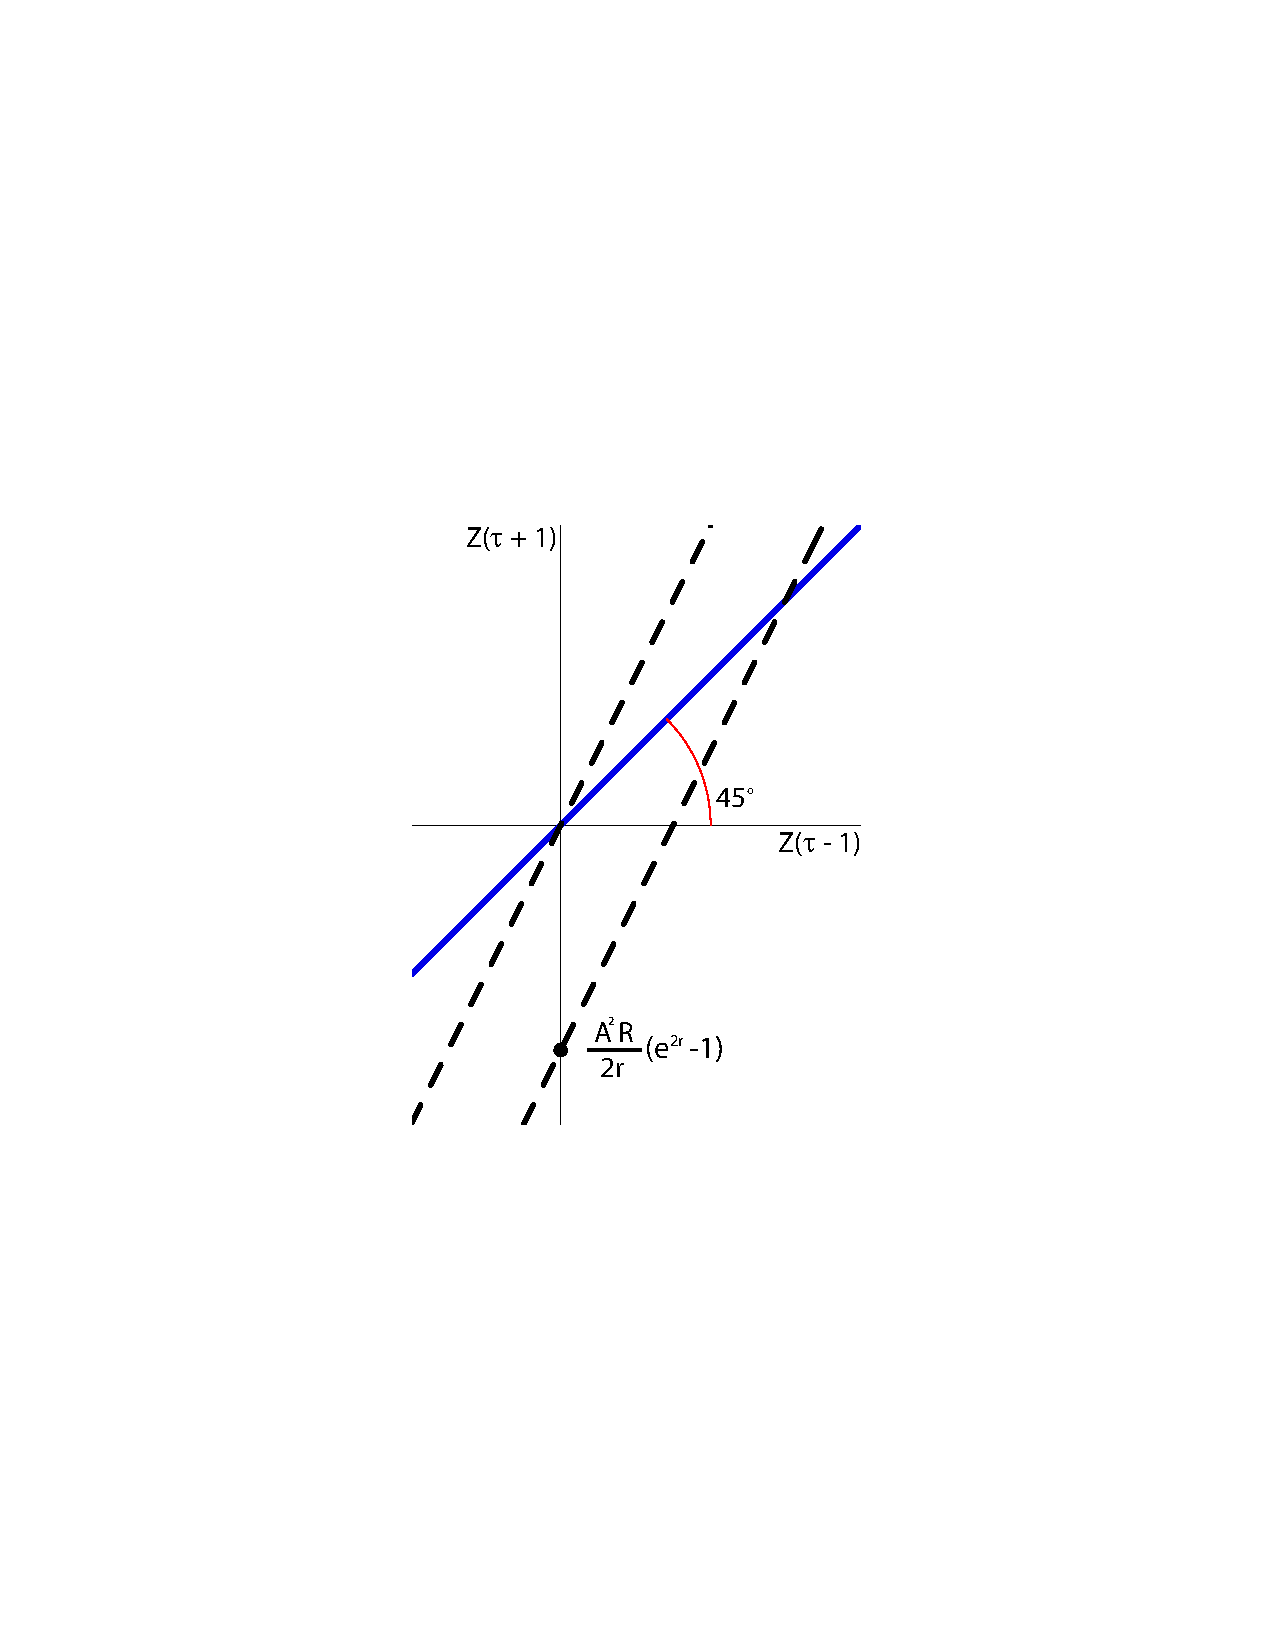
\includegraphics[width=3in, height=3in]{Figures/fig-explode-converge.pdf}
\floatfoot{\begin{small}
Note:
\end{small}}
\end{figure}
\end{center}

\indent Apparently, the dynamics of the earnings growth are explosive. However, note that
\begin{eqnarray}
\frac{\partial \left[ E(\tau) - E(\tau - 1) \right] }{\partial \tau} &=& \frac{A^2 R}{2r} \exp{2r(\tau - T)} \left[ \exp^{-2r} - 1 \right] \nonumber \\
&<& 0
\end{eqnarray}
so that even when the growth dynamics of earnings is explosive, the earnings dynamics, $E(t)$, can converge over time.

\subsection{From the Haley-Rosen Specification to the Mincer Equation}
The earnings function in the Haley-Rosen specification actually lead to the Mincer equation. To see that take the log of \eqref{eq:earningspostalpha12} and obtain
\begin{equation}
\ln E(\tau) = \ln \left( \frac{A^2 R}{ 2r} \right) + \ln \tau + \ln \left[ 1 + \frac{\exp^{-2rT} - \exp^{2r(\tau - T)} }{2r \tau} \right]. \label{eq:logs}
\end{equation}

\indent We can approximate around $\tau_{0}$ the second and third terms in \eqref{eq:logs} to obtain
\begin{eqnarray}
\ln(\tau) &\approx& \ln (\tau_{0}) + \frac{1}{\tau_{0}} \left( \tau - \tau_{0} \right) - \frac{1}{\tau_{0}^2} \frac{\left( \tau - \tau_{0} \right)^2}{2!} \nonumber \\
\ln \left[ 1 + \frac{\exp^{-2rT} - \exp^{2r(\tau - T)} }{2r \tau} \right] &\approx& \xi_{0} + \xi_{1} \left( \tau - \tau_{0} \right) + \xi_{2} \frac{\left( \tau - \tau_{0} \right)^2}{2!}
\end{eqnarray}

\noindent for the adequate $\xi_{0}, \xi_{1}, \xi_{2}$. Thus,
\begin{equation}
\ln(\tau) + \ln \left[ 1 + \frac{\exp^{-2rT} - \exp^{2r(\tau - T)} }{2r \tau} \right] \approx \alpha_{0} + \alpha_{1}\left( \tau - \tau_{0} \right) + \alpha_{2} \left( \tau - \tau_{0} \right)^2
\end{equation}

\noindent with $\alpha_{0} \equiv \ln(\tau_{0}) + \xi_{0}, \alpha_{1} \equiv \frac{1}{\tau_{0}} + \xi_{1}, \alpha_{2} \equiv \frac{-\frac{1}{\tau_{0}^2} + \xi_{2}}{2}$. This leads to the so called Mincer equation \citep[see][]{mincer1974schooling}:
\begin{equation}
\ln E(\tau) = k_{0} + k_{1} \tau + k_{2} \tau^2 \label{eq:mincer}
\end{equation}

\noindent where $k_{0} = \alpha_{0} - \tau_{0} \alpha_{1} + \alpha_{2} \tau_{0}^2, k_{2} = \alpha_{2}$. Also, it provides a baseline to compare ``Ben-Porath'' with ``Mincer'' coefficients. Table \ref{table:bpmincer} provides different combinations of the parameters $r, \tau_{0}, T$ that lead to different values of $k_{1}, k_{2}$ that are close to the estimates that \citet{mincer1974schooling} obtains.

\begin{center}
\begin{table}[H]
\begin{threeparttable}
\fontsize{9}{12pt}\selectfont
\caption{The Ben-Porath and the Mincer Coefficients} \label{table:bpmincer}
\centering
\begin{tabular}{ccc|cc}
\multicolumn{3}{c|}{Parameters} & \multicolumn{2}{c}{Ben Porath
Coefficients} \\ \hline\hline $r$ & $\tau _{0}$ & $T$ & $k_{1}$ &
$k_{2}$ \\ \hline $0.0225$ & $29.54$ & $41.43$ & $0.081$ & $-0.0010$
\\ \hline $0.05$ & $25$ & $60$ & $0.0808$ & $-0.0008$ \\ \hline
$0.05$ & $20$ & $65$ & $0.1002$ & $-0.0013$ \\ \hline $0.0675$ &
$24.70$ & $74.77$ & $0.081$ & $-0.0008$ \\ \hline\hline
\multicolumn{3}{c}{Mincer Coefficients} & $0.081$ & $-0.0012$ \\
\hline
\end{tabular}
\begin{tablenotes}
\small
\item Note: the Mincer model or Mincer equation is $\ln ( \text{E} ) =k_{0}+k_{1}\tau +k_{2}\tau^{2}$, where $\tau$ is experience.  
\end{tablenotes}
\end{threeparttable}
\end{table}
\end{center}

Now, if $rT \approx 0$ then $\exp^{-rT} \approx 1$ and \eqref{eq:logs} becomes 
\begin{equation}
\ln E(\tau) \approx \ln \left( \frac{A^2 R}{2r} \right) + \ln \tau + \ln \left[ 1 + \frac{1 - \exp^{2r \tau}}{2 r \tau} \right] \label{eq:intercept}
\end{equation}

\noindent which leads to various observations. The Haley-Rosen specification of the Ben-Porath model implies no economic content for the Mincerian rate of return on post-school investment. Put differently, an extension of \eqref{eq:mincer} which includes post-school investment does not have a structural counterpart. Actually, this model implies that the entire economic content is in the intercept (see \eqref{eq:intercept}.\eqref{eq:intercept} implies that, \textit{caeteris paribus}, schooling has no effect on earnings. \citet{mincer1974schooling} finds that the opposite holds. However, we claim that his finding does not necessarily argue against the Ben-Porath model. It could simply be the case that \citet{mincer1974schooling} does not include ability measures in his estimations, which appear in \eqref{eq:intercept}, and therefore finds a positive coefficient on schooling. 
% Technically, you should never start a sentence with 'however'. You do this quite often, so I didn't change them. People don't always follow this rule, but you want to consider doing so.
 
\section{Generalized Ben-Porath Model} \label{section:generalized}
We now generalize the model in Section \ref{section:baseline} by relaxing the neutrality assumption so that the production function of human capital is more general. We focus our analysis on specialization because the analysis of other conditions is similar to that of Section \ref{section:baseline}. \\

\indent In particular, the law of motion for human capital stock in the generalized Ben-Porath model is

\begin{equation}
\dot{H} = A I^{\alpha} H^{\beta} - \sigma H \label{eq:lawhgen}.
\end{equation}

\noindent So the model in Section \ref{section:baseline} is a particular case of this general formulation when $\alpha = \beta$. To simplify the analysis of the implications of this model, we assume that there is neither discounting nor depreciation, i.e. $r = \sigma = 0$. To ease notation, we neglect the argument $t$ when possible. We analyze this model with a finite horizon.\\
\indent The Hamiltonian of the problem is
\begin{equation}
\mathcal{H} = RH(t) \left(1 - I(t) \right) + \mu(t) \left( A I(t)^{\alpha} H(t)^{\beta} \right)
\end{equation} 

\noindent where $\mu(t)$ defines the shadow price of human capital. The following condition must be satisfied for interior solutions.

\begin{condition} (Optimality Conditions for the Life-Cycle Individual's Problem in the Generalized Ben-Porath Model) \label{condition:optgen}
\begin{eqnarray}
\frac{\partial \mathcal{H} (\cdot)}{\partial I(t)} = 0 &\Leftrightarrow& \mu(t) A \alpha I(t)^{\alpha - 1} H(t)^{\beta} = RH(t) \label{eq:focinvestmentgen} \\
\frac{\partial \mathcal{H} (\cdot)}{\partial H(t)} = - \dot{\mu(t)} &\Leftrightarrow& -R(1 - I(t)) - \beta \mu(t) A I(t)^{\alpha} H(t)^{\beta -1} = \dot{\mu(t)} \label{eq:focstockgen} \\ 
\frac{\partial \mathcal{H} (\cdot)}{\partial \mu(t)} = \dot{H} &\Leftrightarrow& \dot{H(t)} = A I(t)^\alpha H(t)^\beta \label{eq:focmotiongen} \\
\text{Transversality} &:& \lim_{t \rightarrow T} \mu(t) H(t) = 0 \label{eq:foctransversalitygen}
\end{eqnarray}
\end{condition}

\indent Condition \ref{condition:optgen} is equivalent to the Mangasarian sufficient conditions for a global optimum if $\beta \leq 1$ \citep[see][]{mangasarian1966sufficient}.

\subsection{Specialization}
If $\frac{\partial \mathcal{H} (\cdot)}{\partial I(t)} >0$ with $I(t)=1$, the agent would specialize. Thus the condition that guarantees specialization is as follows.

\begin{condition} (Conditions for Specialization in the Generalized Ben-Porath Model) \label{condition:spe}
\begin{eqnarray}
\text{Conditions for Specialization :}
\begin{cases}
H > \left[ \frac{R}{\alpha A \mu} \right]^{\frac{1}{\beta - 1}}, & \beta > 1 \\
1 > \left[ \frac{R}{\alpha A \mu} \right], & \beta = 1 \\
H < \left[ \frac{R}{\alpha A \mu} \right]^{\frac{1}{\beta - 1}}, & \beta < 1. \\
\end{cases}
\end{eqnarray}
\end{condition}

\indent During the period(s) of specialization \eqref{eq:focstockgen}, \eqref{eq:focmotiongen} become 
\begin{eqnarray}
\dot{\mu} &=& - \beta \mu A H^{\beta - 1} \label{eq:focstockgenspe} \\
\dot{H}  &=& A H^{\beta} \label{eq:focmotiongenspe}
\end{eqnarray}

\noindent and we can solve for the dynamics of human capital stock in this region
\begin{eqnarray}
H(t) =
\begin{cases}
c_{0} \exp^{At}, & \beta = 1 \\ 
\left( At + c_{1} \right)^{\frac{1}{1 - \beta}} (1 - \beta)^{\frac{1}{1 - \beta}}, & \beta \neq 1.

\end{cases}
\end{eqnarray}

\noindent The initial condition for the human capital stock leads to $c_{0} = H_{0} $ and $c_{1} = \frac{H_{0}^{1 - \beta}}{1-\beta}$ which implies that
\begin{eqnarray}
H(t) =
\begin{cases}
H_{0} \exp^{At - 1}, & \beta = 1 \\
\left( At + \frac{H_{0}^{\frac{1}{1-\beta}}}{1-\beta} \right)^{\frac{1}{1 - \beta}} \left( 1 - \beta \right)^{\frac{1}{1-\beta}}, & \beta \neq 1. \label{eq:humanspe}
\end{cases}
\end{eqnarray}

\indent Also, we can solve \eqref{eq:focstockgenspe} and find that
\begin{eqnarray}
\mu(t) =
\begin{cases}
k_{0} \exp^{-At}, & \beta = 1 \\
\frac{k_{1}}{(At + c_{1})^{\frac{\beta}{1-\beta}}}, & \beta \neq 1 \label{eq:muspe}
\end{cases}
\end{eqnarray}

\noindent for which there is an exact solution given an initial condition $\mu(0) = \mu_{0}$. This is, we can find $k_{0}, k_{1}$ in \eqref{eq:muspe} provided $\mu_{0} > 0$ (it is a price). In particular, note that $k_{0} = \mu_{0} > 0$ and $k_{1} = \mu_{0} c_{1}^{\frac{\beta}{1-\beta}} > 0$ for $0<\beta<1$.\\
\indent Let $t^*$ denote the time when specialization ends. It must be true that, then, \eqref{eq:focinvestmentgen} holds with strict equality
\begin{equation}
\mu(t^*) A \alpha H(t^*)^{\beta} = RH(t^*)
\end{equation}

\noindent which implies that 
\begin{equation}
t^* = \frac{1}{A} \left( \ln \left[ \frac{A\alpha}{R} + \ln k_{0} \right] \right)
\end{equation}

\noindent for $\beta = 1$. For $\beta \neq 1$, $t^*$ solves
\begin{equation}
\frac{k_{1}}{ \left( At^* + c_{0} \right)^{\frac{\beta}{\beta-1}}} \frac{A \alpha}{R} = \left[ At^* \left( 1 - \beta \right)^{\frac{1}{1 - \beta}} + H_{0}^{1 - \beta} \left( 1 - \beta \right)^{\frac{\beta}{1 - \beta}} \right]^{1 - \beta}.
\end{equation}

\indent To wrap up the discussion we ask if the period of specialization is unique for particular cases.

\begin{claim} (Uniqueness of the Specialization Period)
If the period of specialization exists, it is unique when either when $\beta = 1$ or when $\beta \in [0,1]$. 
\end{claim}

\begin{proof}
In both cases \eqref{eq:muspe} implies that $\dot{\mu(t)} < 0$. Importantly, $\mu(t)$ is the shadow price or value of human capital. Thus, $\dot{I(t)} < 0 $ and, if it exists, the period of specialization is unique.
\end{proof}

 
\section{The Basic Sheshinski Specification: Bang-Bang Equilibria}
The Basic Sheshinski specification is a particular case of the Generalized Ben-Porath model in Section \ref{section:generalized} in which $\alpha = \beta = 1$.
\begin{definition} (Law of Motion for Human Capital Stock in the Basic Sheshinski Specification)
\begin{equation}
\dot{H(t)} = AI(t)H(t) - \sigma H(t).
\end{equation}
\end{definition}

\indent Proceeding as in Section \ref{section:baseline} and Section \ref{section:generalized} we can write down the current value Hamiltonian and obtain the following optimality conditions for the interior solution.

\begin{condition} (Optimality Conditions for the Life-cycle Individual's Problem in the Basic Sheshinski Specification)
\begin{eqnarray}
\frac{\partial \mathcal{H} (\cdot)}{\partial I(t)} = 0 &\Leftrightarrow& \mu(t) \exp^{rt} = \frac{R}{A} \label{eq:focinvestmentshenbasic} \\
\frac{\partial \mathcal{H} (\cdot)}{\partial H(t)} = - \dot{\mu(t)} &\Leftrightarrow& - \exp^{-rt} R(1 - I(t)) - \mu(t) \left( A I(t) - \sigma \right) = \dot{\mu(t)} \label{eq:focstockshenbasic} \\ 
\frac{\partial \mathcal{H} (\cdot)}{\partial \mu(t)} = \dot{H(t)} &\Leftrightarrow& \dot{H(t)} =  A I(t) H(t)- \sigma H(t) \label{eq:focmotionshenbasic} \\
\text{Transversality} &:& \lim_{t \rightarrow T} \mu(t) H(t) = 0 \label{eq:foctransversalityshenbasic}
\end{eqnarray}
\end{condition}

\begin{claim} (Bang-Bang in the Sheshinski Specification) \label{claim:bangbang}
Assume that $\sigma + r < A$ and that there is an initial period of specialization.\footnote{Note that $\sigma + r > A$ implies that $\dot{g(t)} > 0$ and this violates the transversality condition.} Then, the solution to the problem is Bang-Bang, i.e. either $I = 0$ or $I = 1$. 
\end{claim}

\begin{proof}
Define $g(t) = \mu(t) \exp^{rt}$ and use \eqref{eq:focstockshenbasic}, \eqref{eq:foctransversalityshenbasic} to obtain
\begin{eqnarray}
\dot{g} &=& -R + (R - Ag)I + (\sigma + r)g \label{eq:gbasicshen} \\ 
g(T) &=& 0.
\end{eqnarray}

\indent In the specialization period $I(t) = 1$. If $\sigma + r < A$, $\dot{g(t)}<0$. Actually, by \eqref{eq:focinvestmentshenbasic}, as $g(t)$ decreases to $\frac{R}{A}$, $I(t)$ switches from it's upper bound $1$ to its lower bound $0$. Then, with $I(t) = 0$ we can use $g(T) = 0$ and write

\begin{eqnarray}
\dot{g(t)} &=& (\sigma + r)g(t) - R \nonumber \\
&\Rightarrow& \nonumber \\ 
g(t) &=& \frac{R}{\sigma + r} \left[1 - \exp^{(\sigma + r)(t-T)} \right] \label{eq:gshenbasei0}.
\end{eqnarray}

\noindent for which $\dot{g(t)}<0$ as well. Therefore, once $I(t)$ reaches zero, it is never positive again. This formulation has a Bang-Bang solution.
\end{proof}

\indent It follows that the schooling period, if it exists, is unique and at the beginning of the investment cycle. If it does not exist the individual does not invest at all in human capital. Figure~\ref{fig:bangbang} is a graphical representation of Claim~\ref{claim:bangbang}. 

\begin{center}
\begin{figure}[H]
\caption{Bang-Bang Equilibrium in the Basic Sheshinski Specification} \label{fig:bangbang}
\centering
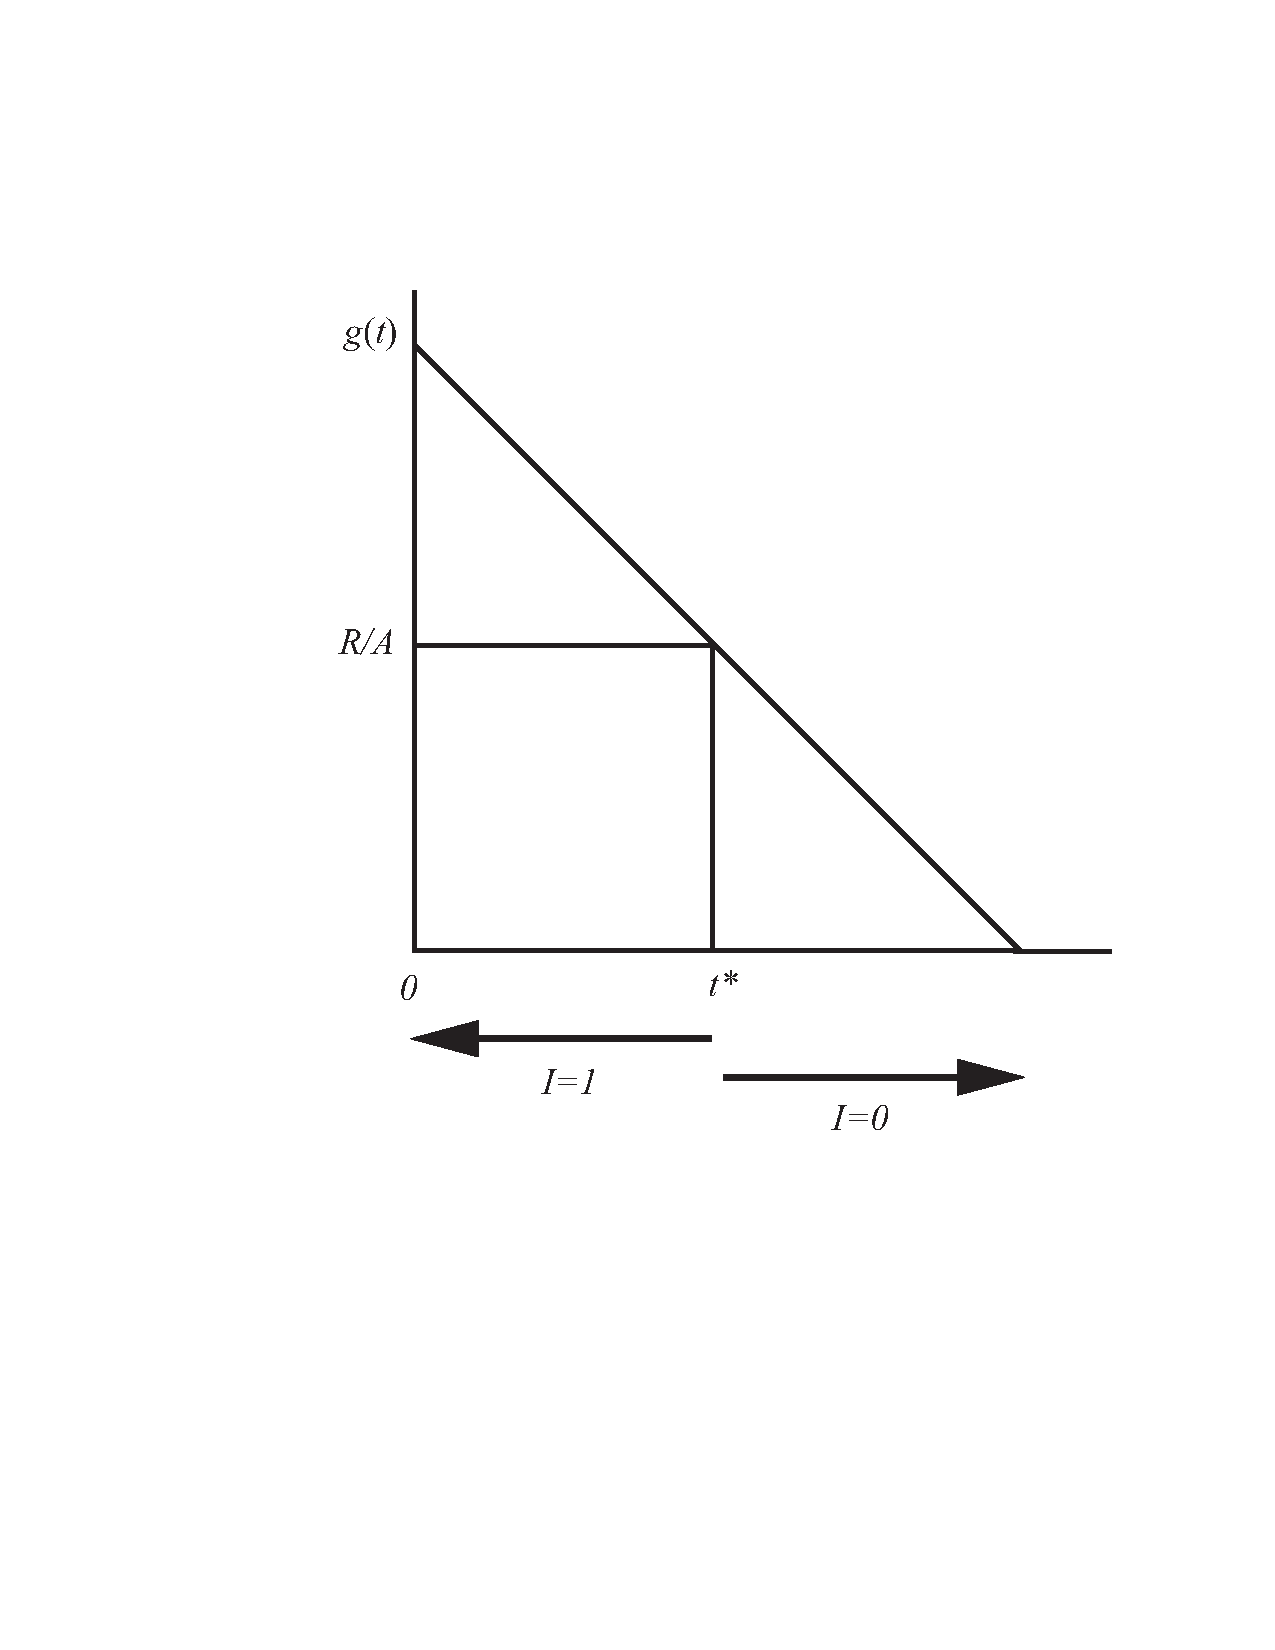
\includegraphics[width=3.5in, height=3.5in]{Figures/fig-shesh-rule.pdf}
\floatfoot{\begin{small}
Note:
\end{small}}
\end{figure}
\end{center}

\indent We can actually solve for $t^*$, the length of the schooling period, using the fact that $g(t^*) = \frac{R}{A} $ by \eqref{eq:focinvestmentshenbasic} and $g(t^*) = \frac{R}{\sigma + r} \left[1 - \exp^{(\sigma + r)(t^*-T)} \right]$ by \eqref{eq:gshenbasei0}:
\begin{eqnarray}
\frac{R}{A} &=& \frac{R}{\sigma + r} \left[1 - \exp^{(\sigma + r)(t^*-T)} \right] \nonumber \\
&\Leftrightarrow& \nonumber \\ 
t^* &=& \frac{1}{\sigma + r} \ln \frac{A - (\sigma + r) }{A} + T.
\end{eqnarray}

\indent Thus, (i) longer life horizons imply more schooling, $\frac{\partial t^*}{\partial T} > 0$; (ii) greater depreciation implies less schooling, $\frac{\partial t^*}{\partial \sigma} < 0$; (iii) higher relative impatience implies less schooling, $\frac{\partial t^*}{\partial r} < 0$; (iv) higher productivity implies more schooling, $\frac{\partial t^*}{\partial A} > 0$; (v) initial human capital does not affect schooling, $\frac{\partial t^*}{\partial H_{0}} = 0$.

\subsection{From the Basic Sheshinski Specification to the Mincer Equation}
Assume that there is a period of specialization. From \eqref{eq:focmotiongenspe} we know that in the period $[0,t^*]$
\begin{eqnarray}
\dot{H(t)} &=& (A - \sigma)H(t) \nonumber \\
&\Rightarrow& \nonumber \\ 
H(t) &=& H_{0} \exp^{(A - \sigma)t}.
\end{eqnarray}

\noindent At $t^*$, actually, $I(t) = 0$ so earnings are $Y(t) = R H(t^*)$ Then,
\begin{equation}
\ln Y(t^*) = \ln(RH_{0}) + (A - \sigma)t^*.
\end{equation} 
\noindent According to this model, the returns to schooling, $A-\sigma$, are given by the productivity of human capital less the human capital depreciation rate.  

\section{The Modified Sheshinski Specification}
The last variation of the Ben-Porath model we consider allows for human capital investment cycles. This is, it allows for investment in human capital stock to happen in different episodes.\\
\begin{definition} (Law of Motion for Human Capital in the Modified Sheshinski Specification)\\
\begin{equation}
\dot{H} = AI - \sigma H. \label{eq:modshenlaw}
\end{equation}
\end{definition}

\indent Note that the human capital production function does not depend on $H(t)$. The optimality conditions for an interior solution in this model are the following.
\begin{condition} (Optimality Condition for the Life-cycle Individual's Problem in the Modified Sheshinski Specification)
\begin{eqnarray}
\frac{\partial \mathcal{H} (\cdot)}{\partial I(t)} = 0 &\Leftrightarrow& \mu \exp^{rt} = \frac{RH}{A} \label{eq:focinvestmentmodsehn} \\
\frac{\partial \mathcal{H} (\cdot)}{\partial H(t)} = - \dot{\mu(t)} &\Leftrightarrow& \dot{\mu} = \mu \sigma - \exp^{-rt} R (1 - I) \label{eq:focstockmodshen} \\ 
\frac{\partial \mathcal{H} (\cdot)}{\partial \mu(t)} = \dot{H(t)} &\Leftrightarrow& \dot{H(t)} = AI - \sigma H \label{eq:focmotionmodshen} \\
\text{Transversality} &:& \lim_{t \rightarrow T} \mu(t) H(t) = 0. \label{eq:foctransversalitymodshen}
\end{eqnarray}
\end{condition}

\subsection{No Depreciation: a Schooling Model}
\indent Define $g(t) = \mu(t) \exp^{rt}$ and use \eqref{eq:focstockmodshen} to obtain
\begin{equation}
\dot{g} = g(\sigma + r) - R(1 - I). \label{eq:gmodshen}
\end{equation}

\noindent Let $\sigma = 0 $. Then $\dot{g} = -R(1 - I) + rg$. And $\dot{H} = A$ when $I=1$. So the solution for the human capital trajectory when $I = 1$ is
\begin{equation}
H(t) = At + H_{0} \label{eq:humancapshenmod}.
\end{equation} 

\noindent At $t = 0$, $I = 1$ if $g(0) > \frac{R}{A} H_{0}$. Importantly, $I = 1$ implies that $\dot{g(t)} = r g(t) > 0$. As $t$ grows, the return for gross investment grows because the payoff period gets closer. $I = 1$ cannot be a solution forever because the agent receives no earnings if she invests all of the time during the complete life-cycle.\\
\begin{claim} (Uniqueness of the Period of Specialization in the Modified Sheshinski Specification with no Depreciation)
If the specialization period exists, then it is unique.
\end{claim}

\begin{proof}
Based on \eqref{eq:focinvestmentmodsehn}, if a specialization period exists and if $g(t) - \frac{RH(t)}{A}$ is strictly decreasing overtime, then the specialization period must occur at the beginning of the life cycle and is unique. In the following we show that $\dot{g(t)} - \frac{R}{A}\dot{H(t)} < 0$.\\

\indent Given that $\dot{g(t)} = rg(t) - R(1-I(t))$ and $g(T)=0$, we have:
\begin{eqnarray}
g(t) = R \int_t^T (1-I(s)) \exp^{r(t-s)} ds \label{eq:gshendisc}
\end{eqnarray}

\noindent Then taking the derivative with respect to time gives:
\begin{eqnarray}
\dot{g(t)} = R \left[ -1 + I(t) + r\int_t^T (1-I(s)) \exp^{r(t-s)} ds \right] 
\end{eqnarray}

\noindent Together with \eqref{eq:modshenlaw}, we have:
\begin{eqnarray}
\dot{g(t)} - \frac{R}{A} \dot{H(t)} &=& -R + Rr\int_t^T (1-I(s)) \exp^{r(t-s)} ds\\
&\leq & -R + Rr\int_t^T \exp^{r(t-s)} ds \\
&=& -R\exp^{r(t-T)} \\
&<& 0,  
\end{eqnarray}

\noindent where the first inequality follows from setting $I(\tau)=0$.
\end{proof}

\indent Finally, to compute the optimal schooling length, $t^*$, note that \eqref{eq:focinvestmentmodsehn} holds with strict equality at $t^*$ and \eqref{eq:humancapshenmod} is valid so that
\begin{equation}
g(t^*) = \frac{R}{A} \left( A t^* + H_{0} \right). 
\end{equation}

\noindent \eqref{eq:gshendisc} is also valid for $t^*$. Then,
\begin{equation}
\left( 1 - \exp^{r(t^*-T)} \right) = \frac{r}{A} \left( A t^* + H_{0} \right)
\end{equation}

\noindent and thus $\frac{\partial t^*}{\partial H_{0}} < 0, \frac{\partial t^*}{\partial A}> 0$ and $\frac{\partial t^*}{\partial r} < 0$ as in the model of Section \ref{section:baseline}. 
 
\subsection{Depreciation} \label{section:cycles}
Let us give some conditions under which human capital investment would have different episodes over the life cycle. First assume that $g(0) > \frac{H_{0} R}{A}$ so that there is a specialization period to begin with. We can solve \eqref{eq:focmotionmodshen} and \eqref{eq:gmodshen} to obtain
\begin{eqnarray}
H(t) &=& \left[ H_{0} - \frac{A}{\sigma} \right] \exp^{- \sigma t} + \frac{A}{\sigma} \nonumber \\
g(t) &=& g_{0} \exp^{(r + \sigma)t} \label{eq:gmodshent1} \nonumber
\end{eqnarray}

\noindent with $g_{0} > 0$. Once the solution becomes interior, $g(t) = \frac{R}{A} H(t)$ by \eqref{eq:focinvestmentmodsehn}. Assume that  $\sigma < \frac{A}{H_{0}}$ so that $\dot{H(0)} > 0$. Then, graphically,

\begin{center}
\begin{figure}[H]
\caption{Return to Gross Investment in Human Capital in the Modified Sheshinski Specification}
\centering
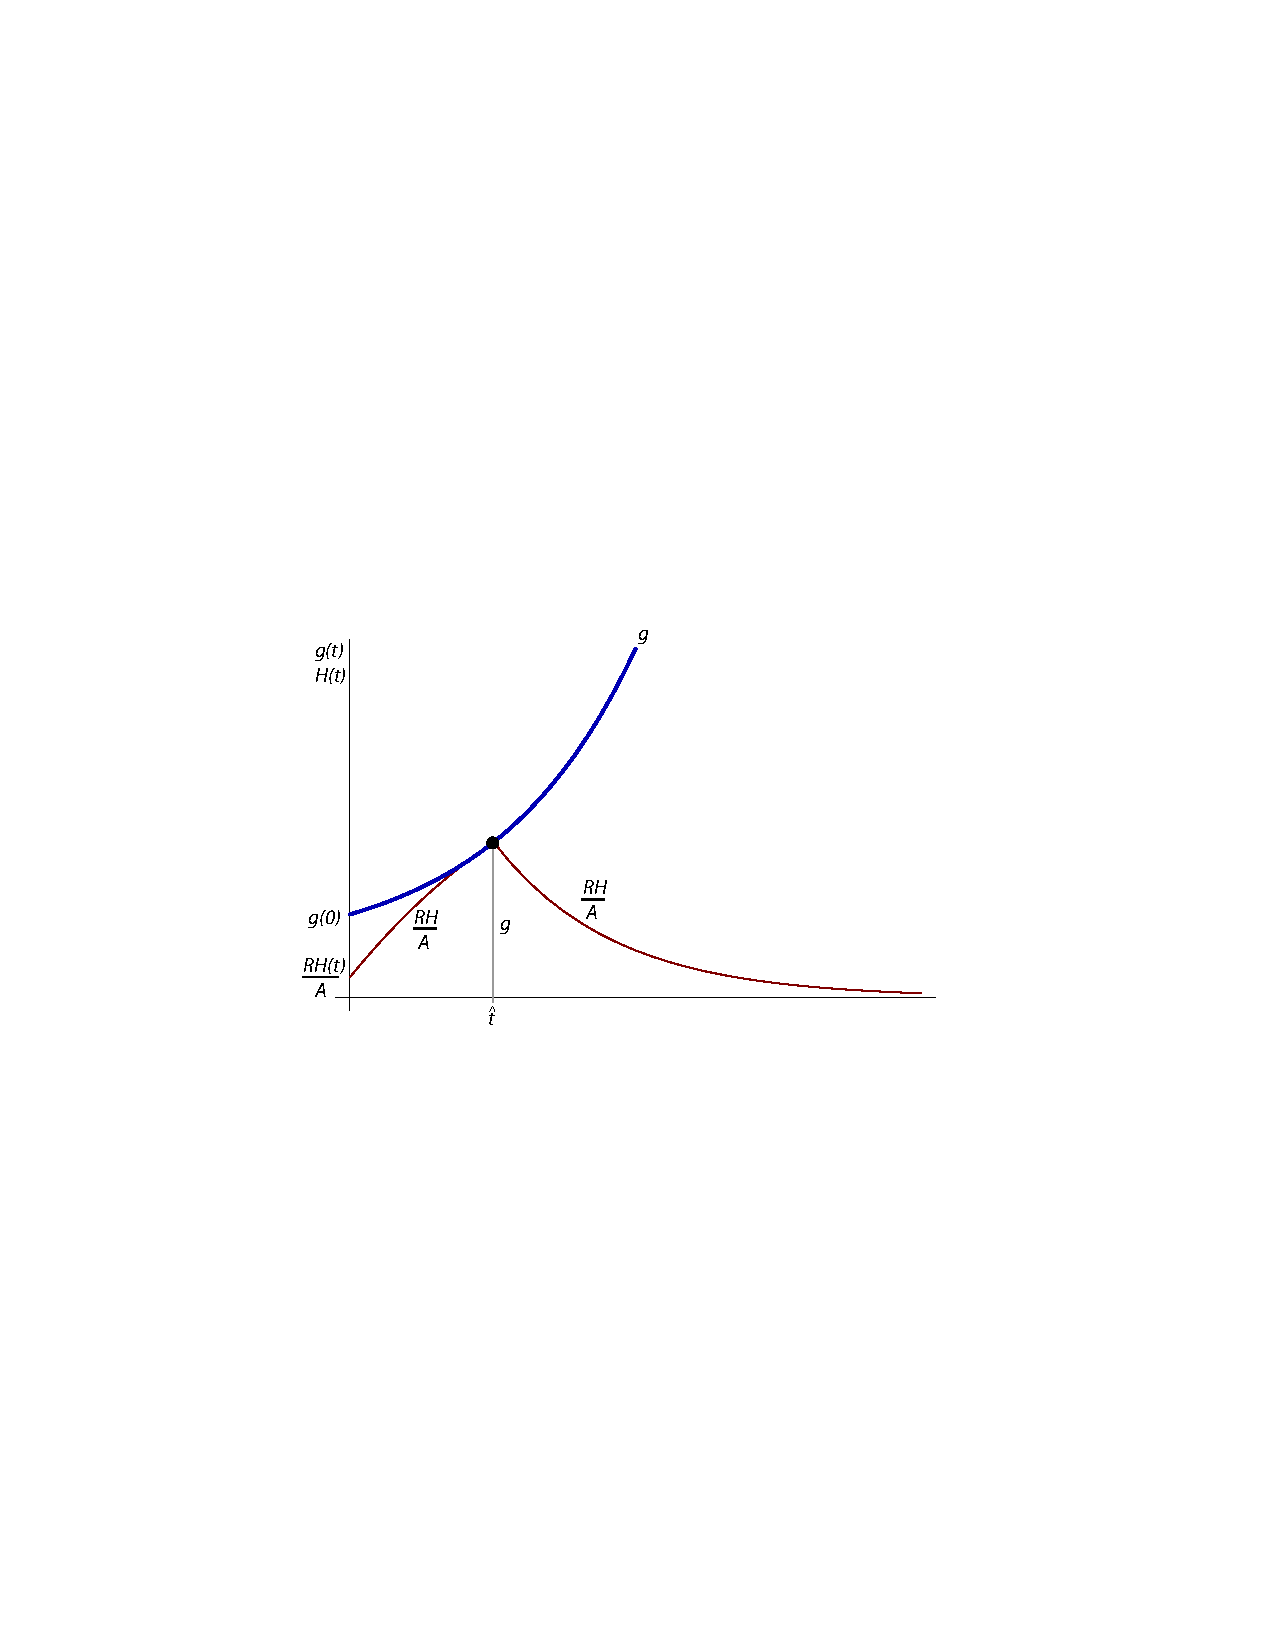
\includegraphics[width=4.5in, height=3.5in]{Figures/fig-shesh-for-intersection.pdf}
\floatfoot{\begin{small}
Note:
\end{small}}
\end{figure}
\end{center}

\indent Let $t_{1}$ denote the time in which the first period of specialization ends. If the solution ``bangs-out'' to $I=0$ we can use \eqref{eq:gmodshen} and \eqref{eq:modshenlaw} to get
\begin{eqnarray}
\dot{g} &=& (\sigma + r)g - R \nonumber \\
H(t) &=& H(t_{1}) \exp^{-\sigma(t - t_{1})} 
\end{eqnarray}

\noindent for $t_{1} < t < t_{2}$. Likewise, we can define a period $t_{2}$ in which the solution ``bangs-in'' again and so on. Graphically,

\begin{center}
\begin{figure}[H]
\caption{Human Capital Investment Episodes in the Modified Sheshinski Specification} \label{figure:multi}
\centering
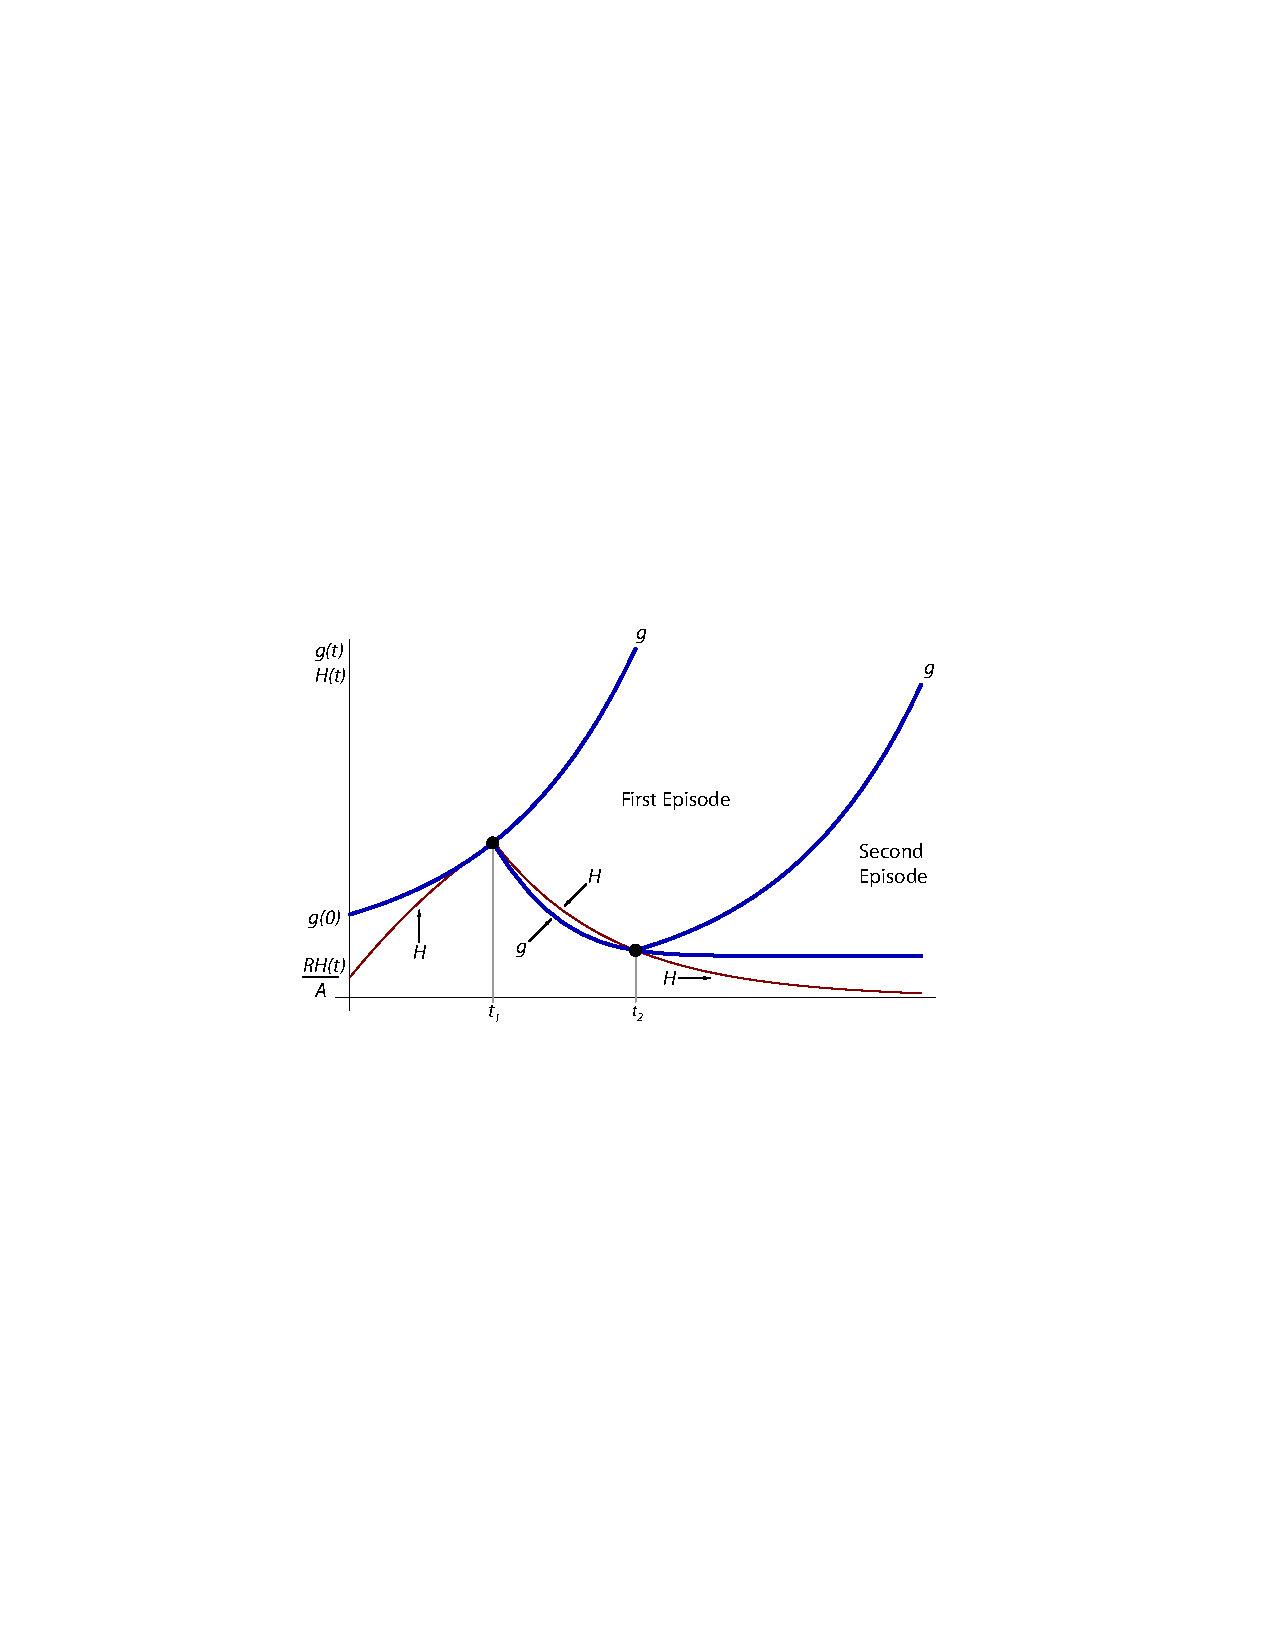
\includegraphics[width=4.5in, height=3.5in]{Figures/fig-shesh-one-traj.pdf}
\floatfoot{\begin{small}
Note:
\end{small}}
\end{figure}
\end{center}

\indent In $t < t_{1}$, $I = 1$ implies $\dot{g} > 0$. $g$ needs to decrease for the problem to respect the transversality condition. Thus, in the neighborhood of $t_{1}$ it has to be that $\dot{g(t_{1})} < \frac{R \dot{H(t_{1})}}{A}$ (see Figure \eqref{figure:multi}). If we take the expression from the right of $g(t_{1})$ this requires
\begin{eqnarray}
- R (\sigma + r) g(t_{1}) &<& \frac{R \dot{H(t_{1})}}{A} \nonumber \\
&=& \frac{- \sigma R H(t_{1})}{A} \nonumber \\
&=& -\sigma g(t_{1}) \nonumber \\
&\Leftrightarrow& \nonumber \\
g(t_{1}) &<& \frac{R}{r}.  
\end{eqnarray}

\noindent We can follow analogous reasoning to construct conditions under which human capital investment happens in different episodes during the life-cycle.\\
\indent To wrap up this section, note that we have an initial period of specialization if $g_{0} > \frac{R H_{0}}{A}$. At $t=0$, however, it should be the case that the slope of $\frac{R H_{0}}{A}$ exceeds $\dot{g}$. Otherwise the expressions for $g$ in the specialization period and the ``interior'' case do not intersect and the solution violates the transversality condition. This implies that $R \left[ 1 - \frac{\sigma H_{0}}{A} \right] > g_{0}(\sigma + r)$. High initial levels of human capital, low productivity, high discount, high depreciation, and low returns to human capital rule out an initial specialization period. Suppose the conditions described above hold so that specialization happens. We cannot show that $g(t_{3}) < g(t_{1})$ so that it is better to accumulate ``all the human capital required for life'' in the first period of specialization. This is what we call cycling in the investment on human capital and it is a consequence of depreciation.












\clearpage
\bibliographystyle{chicago}
\bibliography{BibtexFiles/BenPorath}



\end{document}
